%%%%%%%%%%%%%%%%%%%%%%%%%%%%%%%%%%%%%%%%%
% Beamer Presentation
% LaTeX Template
% Version 1.0 (10/11/12)
%
% This template has been downloaded from:
% http://www.LaTeXTemplates.com
%
% License:
% CC BY-NC-SA 3.0 (http://creativecommons.org/licenses/by-nc-sa/3.0/)
%
%%%%%%%%%%%%%%%%%%%%%%%%%%%%%%%%%%%%%%%%%

%----------------------------------------------------------------------------------------
%	PACKAGES AND THEMES
%----------------------------------------------------------------------------------------

\documentclass{beamer}

\mode<presentation> {

% The Beamer class comes with a number of default slide themes
% which change the colors and layouts of slides. Below this is a list
% of all the themes, uncomment each in turn to see what they look like.

%\usetheme{default}
%\usetheme{AnnArbor}
%\usetheme{Antibes}
%\usetheme{Bergen}
%\usetheme{Berkeley}
%\usetheme{Berlin}
%\usetheme{Boadilla}
%\usetheme{CambridgeUS}
%\usetheme{Copenhagen}
%\usetheme{Darmstadt}
%\usetheme{Dresden}
%\usetheme{Frankfurt}
%\usetheme{Goettingen}
%\usetheme{Hannover}
%\usetheme{Ilmenau}
%\usetheme{JuanLesPins}
%\usetheme{Luebeck}
\usetheme{Madrid}
%\usetheme{Malmoe}
%\usetheme{Marburg}
%\usetheme{Montpellier}
%\usetheme{PaloAlto}
%\usetheme{Pittsburgh}
%\usetheme{Rochester}
%\usetheme{Singapore}
%\usetheme{Szeged}
%\usetheme{Warsaw}

% As well as themes, the Beamer class has a number of color themes
% for any slide theme. Uncomment each of these in turn to see how it
% changes the colors of your current slide theme.

%\usecolortheme{albatross}
%\usecolortheme{beaver}
%\usecolortheme{beetle}
%\usecolortheme{crane}
%\usecolortheme{dolphin}
%\usecolortheme{dove}
%\usecolortheme{fly}
%\usecolortheme{lily}
%\usecolortheme{orchid}
%\usecolortheme{rose}
%\usecolortheme{seagull}
%\usecolortheme{seahorse}
%\usecolortheme{whale}
%\usecolortheme{wolverine}

%\setbeamertemplate{footline} % To remove the footer line in all slides uncomment this line
%\setbeamertemplate{footline}[page number] % To replace the footer line in all slides with a simple slide count uncomment this line

%\setbeamertemplate{navigation symbols}{} % To remove the navigation symbols from the bottom of all slides uncomment this line
}

\usepackage{graphicx} % Allows including images
\usepackage{booktabs} % Allows the use of \toprule, \midrule and \bottomrule in tables

%----------------------------------------------------------------------------------------
%	TITLE PAGE
%----------------------------------------------------------------------------------------

\title[GBMs Optimization using Optuna]{Study on Gradient Boosting Algorithms and
Hyperparameter Optimization using Optuna} % The short title appears at the bottom of every slide, the full title is only on the title page

\author{João Manoel Herrera Pinheiro} % Your name
\institute[EESC] % Your institution as it will appear on the bottom of every slide, may be shorthand to save space
{
University of São Paulo \\ % Your institution for the title page
\medskip
\textit{joaomh@protonmail.com} % Your email address
}
\date{\today} % Date, can be changed to a custom date

\begin{document}

\begin{frame}
\titlepage % Print the title page as the first slide
\end{frame}

\begin{frame}
\frametitle{Overview} % Table of contents slide, comment this block out to remove it
\tableofcontents % Throughout your presentation, if you choose to use \section{} and \subsection{} commands, these will automatically be printed on this slide as an overview of your presentation
\end{frame}

%----------------------------------------------------------------------------------------
%	PRESENTATION SLIDES
%----------------------------------------------------------------------------------------

%------------------------------------------------
\section{Introduction - 5min} % Sections can be created in order to organize your presentation into discrete blocks, all sections and subsections are automatically printed in the table of contents as an overview of the talk
%------------------------------------------------
\subsection{Supervised Machine Learning}
\begin{frame}
\frametitle{Supervised $\times$ Unsupervised $\times$ Reinforcement}
\begin{figure}[h]
 \centering
 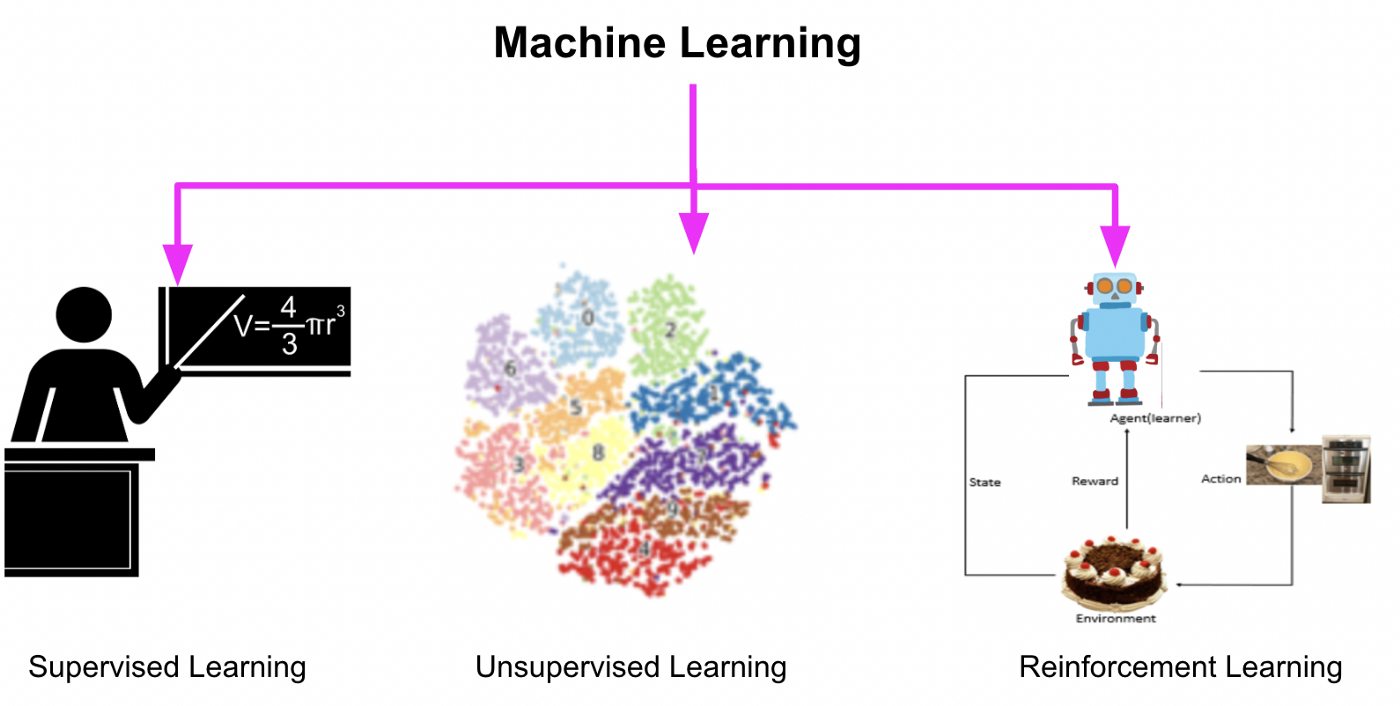
\includegraphics[scale=0.25]{super_intro.png}
\end{figure}
\end{frame}
\begin{frame}
\frametitle{Supervised $\times$ Unsupervised $\times$ Reinforcement}
\begin{block}{Supervised Learning}
In supervised learning, the AI model is trained based on the given input and its expected output. Decision trees, linear regression, KNN, Random Forest. Image detection, Population growth prediction
\end{block}
\begin{block}{Unsupervised Learning}
In unsupervised learning, the AI model is trained only on the inputs, without their labels. The model classifies the input data into classes that have similar features. K-means,DBSCAN, HCA. Customer segmentation, feature elicitation, targeted marketing.
\end{block}
\begin{block}{Reinforcement Learning}
In reinforcement learning, the AI model tries to take the best possible action in a given situation to maximize the total profit. The model learns by getting feedback on its past outcomes. Deep Learning, Q-Learning, Markov decision process. Self Driving Cars.
\end{block}
\end{frame}
\subsection{Machine Learning Steps}
\begin{frame}
\frametitle{Machine Learning Steps}
\begin{itemize}
\item Understand the Problem
\item Collecting Data
\item Preparing the Data
\item Choosing a Model
\item Training the Model
\item Evaluating the Model
\item Tuning the Model
\item Making Predictions 
\end{itemize}
\end{frame}
\begin{frame}
\frametitle{Bias–Variance Tradeoff}
\begin{figure}
     \begin{subfigure}
         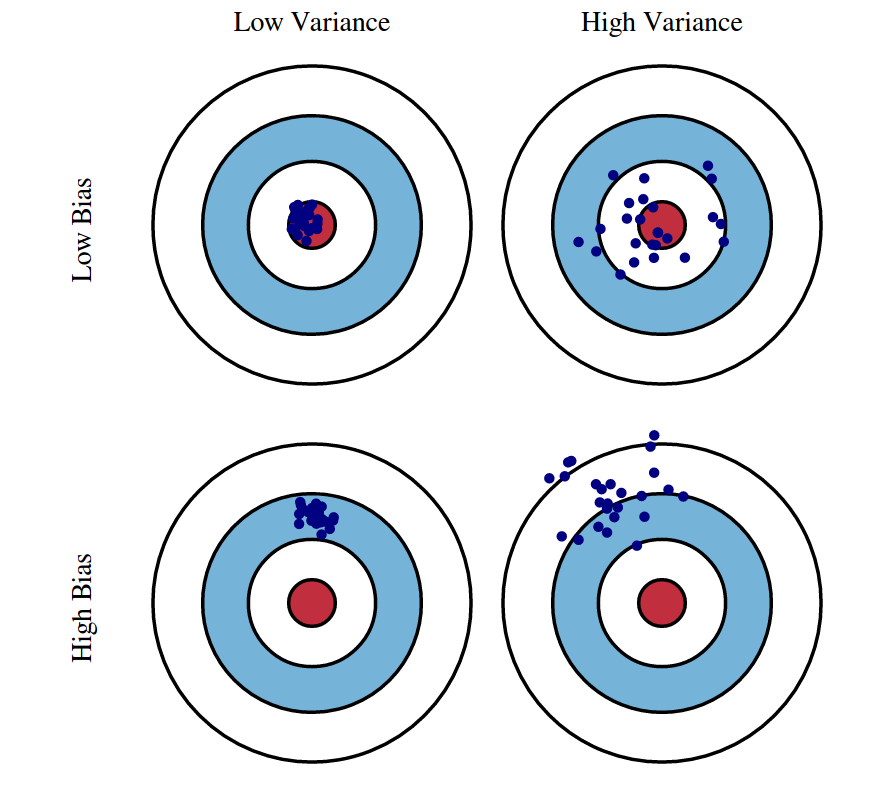
\includegraphics[scale=0.2]{bias_1.png}
     \end{subfigure}
     \begin{subfigure}
         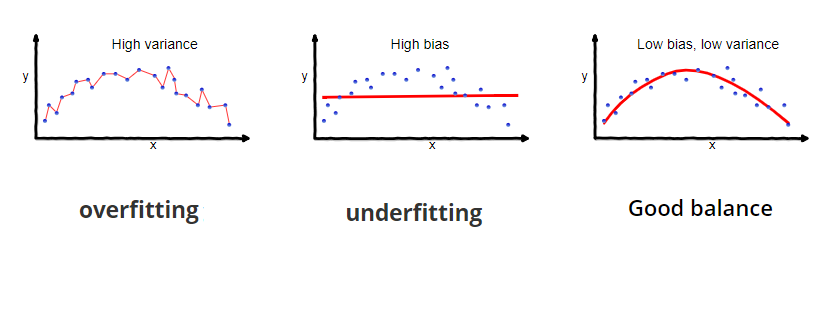
\includegraphics[scale=0.25]{bias_2.png}
     \end{subfigure}
\end{figure}
\end{frame}
\begin{frame}
\frametitle{Bias–Variance Tradeoff}
\begin{block}{Bias}
Bias is the difference between the average prediction of our model and the correct value which we are trying to predict. Model with high bias pays very little attention to the training data and oversimplifies the model. It always leads to high error on training and test data.
\end{block}
\begin{block}{Variance}
Variance is the variability of model prediction for a given data point or a value which tells us spread of our data. Model with high variance pays a lot of attention to training data and does not generalize on the data which it hasn’t seen before. As a result, such models perform very well on training data but has high error rates on test data.
\end{block}
\end{frame}
\begin{frame}
\frametitle{Bias–Variance Tradeoff}
\begin{block}{Underfitting}
Happens when a model unable to capture the underlying pattern of the data. These models usually have high bias and low variance.
\end{block}
\begin{block}{Overfitting}
Happens when our model captures the noise along with the underlying pattern in data. It happens when we train our model a lot over noisy dataset. These models have low bias and high variance.
\end{block}
\end{frame}

\begin{frame}
\frametitle{Train-Validation-Test}
\begin{figure}[h]
 \centering
 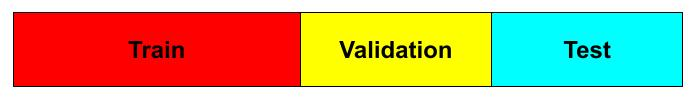
\includegraphics[scale=0.3]{train-test.jpg}
\end{figure}
\end{frame}
\begin{frame}
\frametitle{Train-Validation-Test}
\begin{block}{Train}
Training Dataset: The sample of data used to fit the model.The model sees and learns from this data.
\end{block}
\begin{block}{Validation}
Validation Dataset: The sample of data used to provide an unbiased evaluation of a model fit on the training dataset while tuning model hyperparameters.
\end{block}
\begin{block}{Test}
Test Dataset: The sample of data used to provide an unbiased evaluation of a final model fit on the training dataset.
\end{block}
\end{frame}
\subsection{Binary Classification}
\begin{frame}
\frametitle{Binary Classification}
\begin{block}{Binary Classification}
Binary classification is a supervised learning algorithm that categorizes new observations into one of two classes. Often 0 or 1.
\end{block}
\begin{figure}[h]
 \centering
 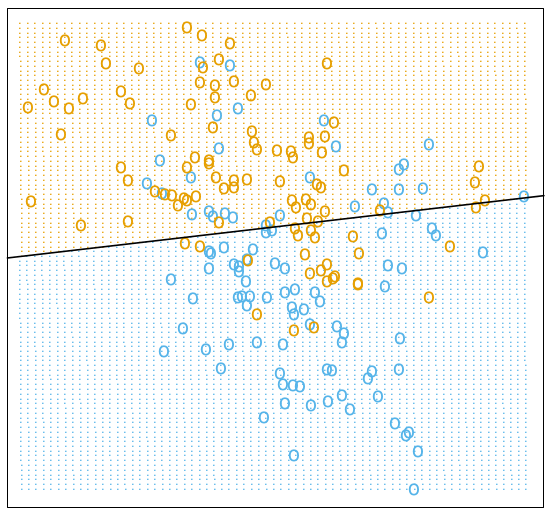
\includegraphics[scale=0.25]{classificacao_hastie_ex.png}
\end{figure}
\end{frame}
\subsection{Validation Metrics}
\begin{frame}
\frametitle{Validation Metrics:}
\begin{block}{AUC}
AUC functionally measures how well-ordered results are in accordance with true class membership. Higher the AUC, the better the model is at predicting 0 classes as 0 and 1 classes as 1.
\end{block}
\begin{block}{Logloss}
Log-loss is indicative of how close the prediction probability is to the corresponding actual/true value (0 or 1 in case of binary classification). The more the predicted probability diverges from the actual value, the higher is the log-loss value.
\end{block}
\begin{block}{KS}
The KS statistic for two samples is simply the highest distance between their two CDFs, so if we measure the distance between the positive and negative class distributions, we can have another metric to evaluate classifiers.
\end{block}
\end{frame}
\begin{frame}
\frametitle{Validation Metrics: AUC}
\begin{block}{ROC}
The ROC curve is plotted with the True Positive Rate, or Sensitivity, against False Positive Rate, or 1 - Specificity.

\end{block}
\begin{figure}[h]
 \centering
 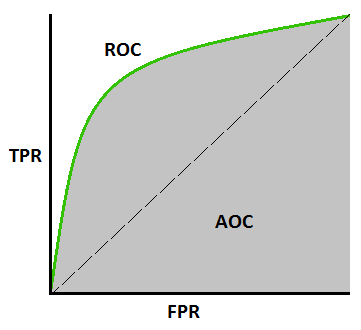
\includegraphics[scale=0.25]{rock.png}
\end{figure}
\begin{gather*}
    Roc_{y}(\mathcal{T}) =Sensitivity= TPR_{\mathcal{T}} = \frac{TP_{\mathcal{T}}}{TP_{\mathcal{T}} + FN_{\mathcal{T}}} \\
    Roc_{x}(\mathcal{T}) =1 - Specificity= FPR_{\mathcal{T}} = \frac{FP_{\mathcal{T}}}{FP_{\mathcal{T}} + TN_{\mathcal{T}}}
\end{gather*}
\end{frame}
\begin{frame}
\frametitle{Validation Metrics: Logloss}
\begin{block}{Logloss}
Log-loss is indicative of how close the prediction probability is to the corresponding actual/true value (0 or 1 in case of binary classification). The more the predicted probability diverges from the actual value, the higher is the log-loss value.
\end{block}
\begin{figure}[h]
 \centering
 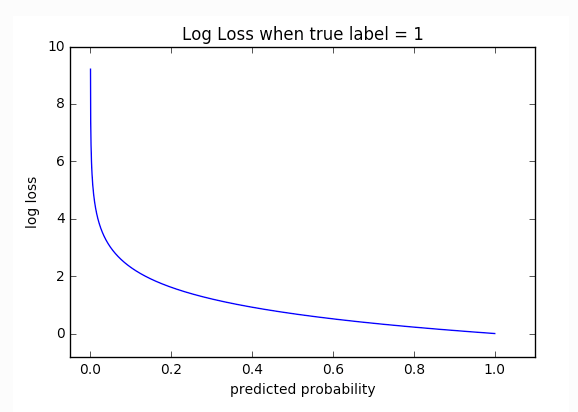
\includegraphics[scale=0.25]{logloss_grap.png}
\end{figure}
\begin{equation*}
    Logloss = -\frac{1}{N}\sum_{i=1}^n[y^{(i)}\log \hat{y}^{(i)} + (1-y^{(i)})\log(1-\hat{y}^{(i)})]
\end{equation*}
\end{frame}
\begin{frame}
\frametitle{Validation Metrics: Kolmogorov-Smirnov Test}
\begin{block}{KS}
The Kolmogorov–Smirnov statistic quantifies a distance between the empirical distribution function of the sample and the cumulative distribution function of the reference distribution, or between the empirical distribution functions of two samples.
\end{block}
\begin{figure}[h]
 \centering
 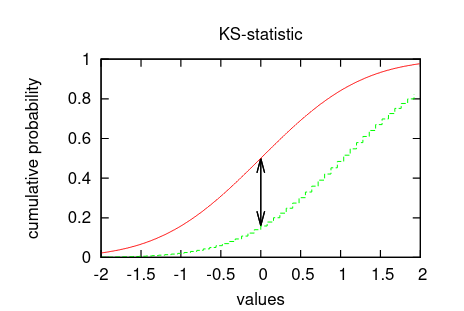
\includegraphics[scale=0.35]{ks_statis.png}
\end{figure}
\begin{equation*}
    KS = \max(TPR - FPR)
\end{equation*}
\end{frame}
\subsection{Shapley Values}
\begin{frame}
\frametitle{Shapley Values}
\begin{block}{SHAP (SHapley Additive exPlanations)}
SHAP is a game theoretic approach to explain the output of any machine learning model. It connects optimal credit allocation with local explanations using the classic Shapley values from game theory and their related extensions
\end{block}
\begin{equation*}
    g(z') = \phi_{0} + \sum_{i=1}^{M} \phi_{i}z'_{i}
\end{equation*}
\end{frame}
\begin{frame}
\frametitle{SHAP}
\begin{figure}[h]
 \centering
 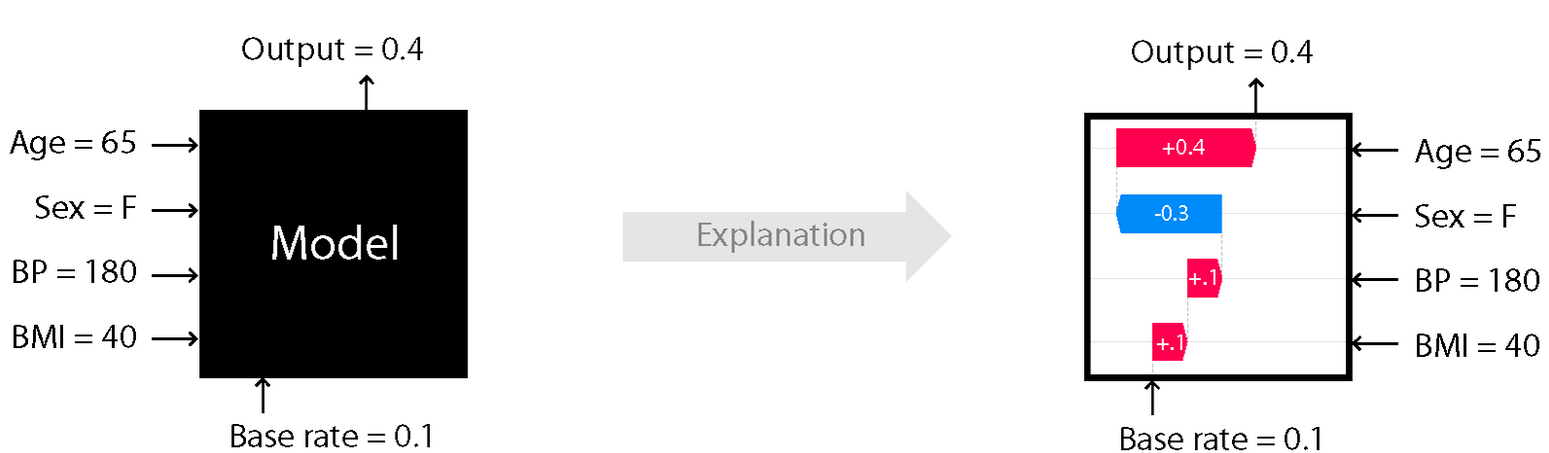
\includegraphics[scale=0.18]{exemplo_shap_black.png}
\end{figure}
\begin{figure}[h]
 \centering
 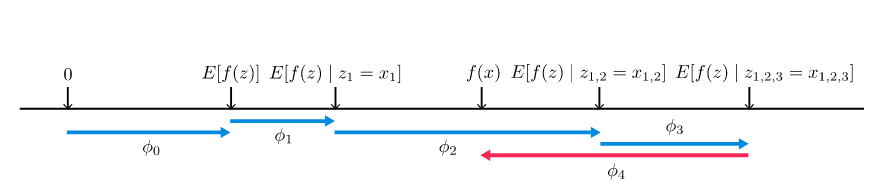
\includegraphics[scale=0.3]{shap_value_artigo.png}
\end{figure}
\end{frame}
% \begin{frame}
% \frametitle{SHAP - Diabetes}
% \begin{figure}[h]
%  \centering
%  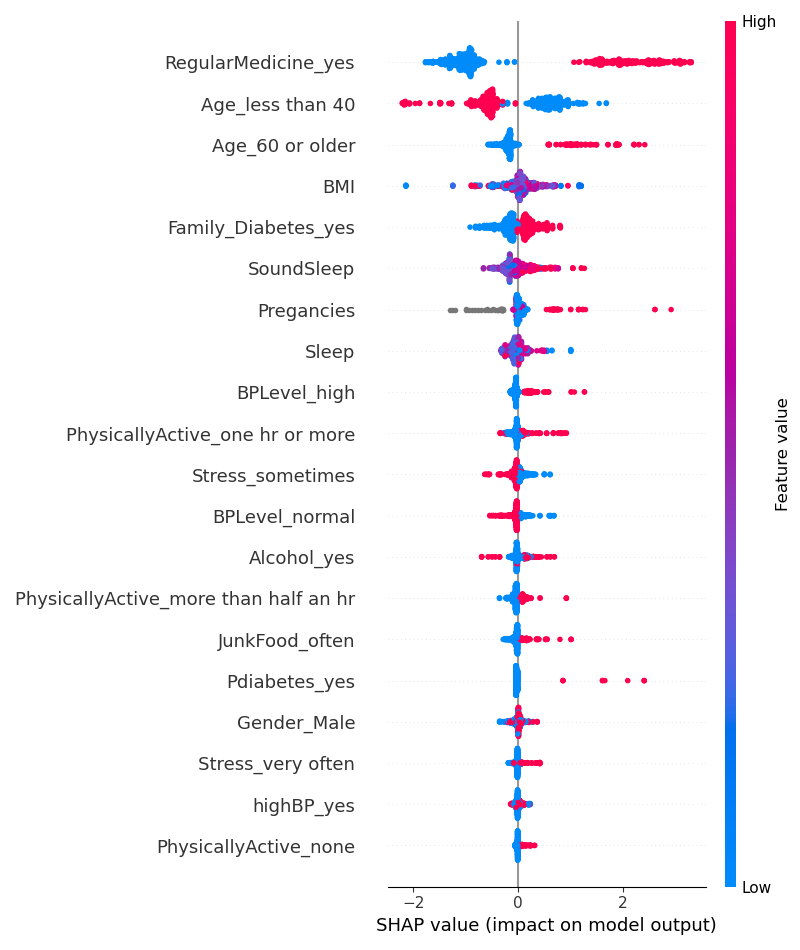
\includegraphics[scale=0.32]{shap_lgbm_diabete.png}
% \end{figure}
% \end{frame}
\section{XGBoost, CatBoost and LightGBM - 5min}
% \subsection{Decision Tree}
% \begin{frame}
% \frametitle{Decision Tree}
% \begin{figure}[h]
%  \centering
%  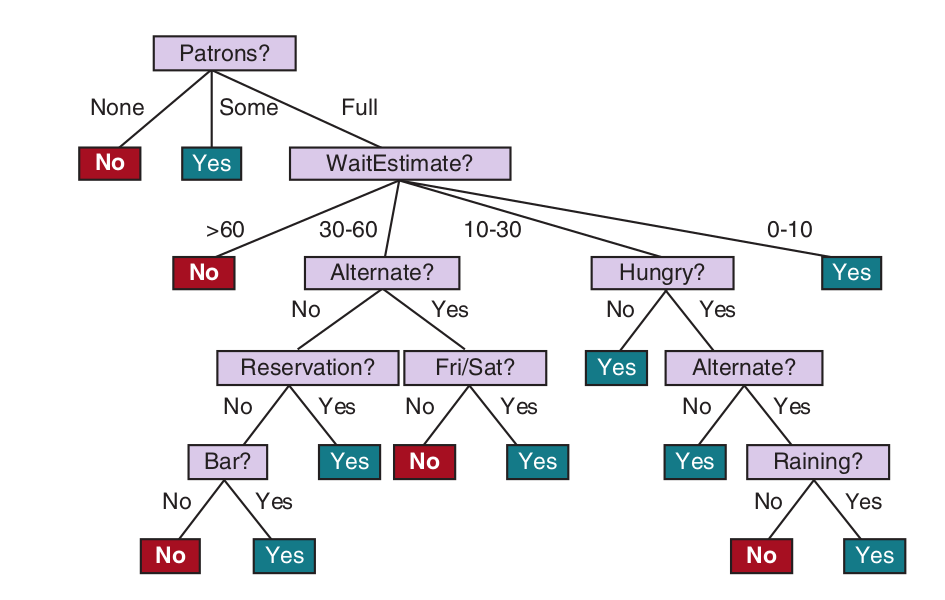
\includegraphics[scale=0.32]{exemplo_arvore.png}
% \end{figure}
% \end{frame}
\subsection{Gradient Boosting}
\begin{frame}
\frametitle{Gradient Boosting}
\begin{block}{Boosting}
 Boosting is a method of converting weak learners into strong learners. In boosting, each new tree is a fit on a modified version of the original data set.
\end{block}
 \begin{figure}[h]
 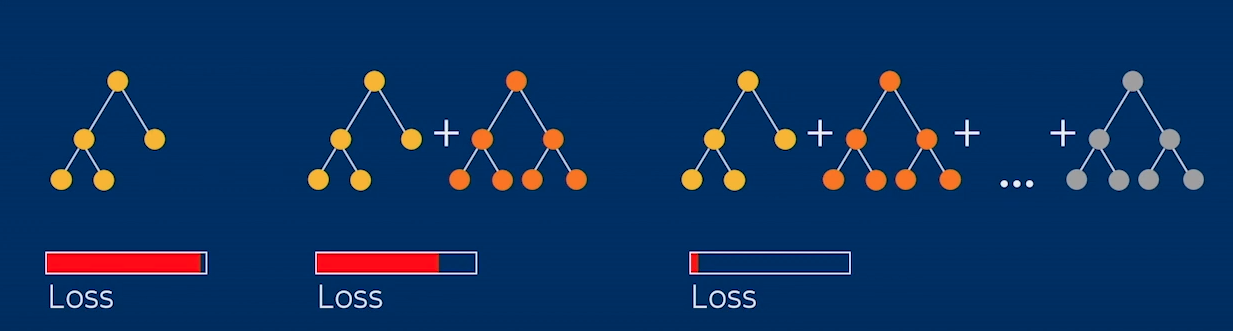
\includegraphics[scale=0.25]{boosting.png}
\end{figure}
\end{frame}
% \begin{equation*}
%     F_m(\mathbf{X}) = F_{m-1}\mathbf({X}) + \eta \Delta_m(X)
% \end{equation*}
\subsection{XGBoost x CatBoost x LightGBM}
\begin{frame}
\frametitle{XGBoost x CatBoost x LightGBM}
 \begin{figure}[h]
 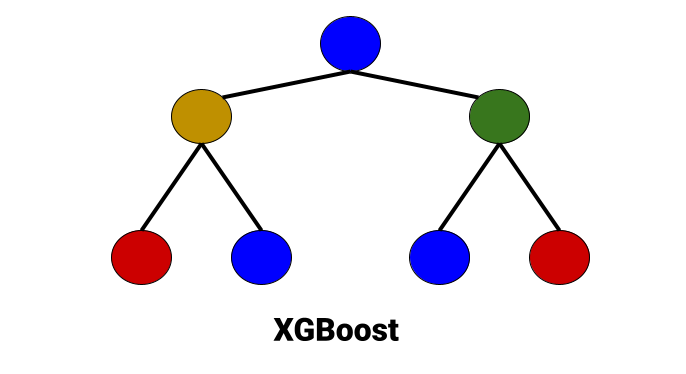
\includegraphics[scale=0.2]{XGboost.png}
  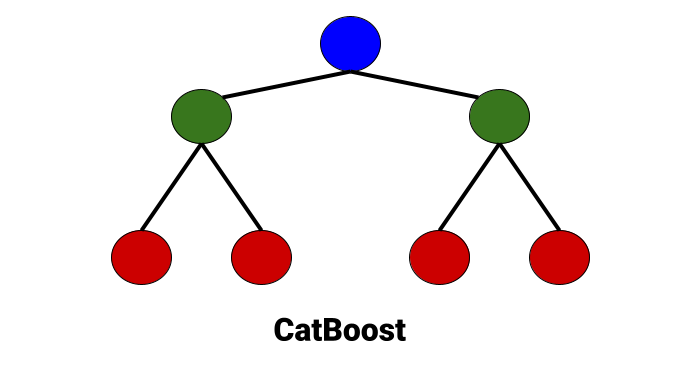
\includegraphics[scale=0.2]{CatBoost.png}
   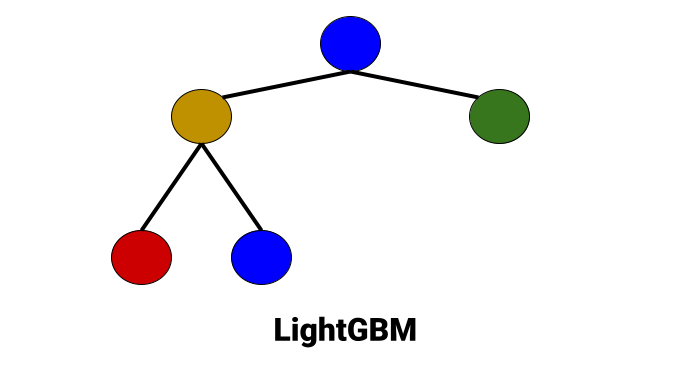
\includegraphics[scale=0.2]{LGBM.png}
\end{figure}
\end{frame}
\begin{frame}
\frametitle{XGBoost x CatBoost x LightGBM}
 \begin{figure}[h]
 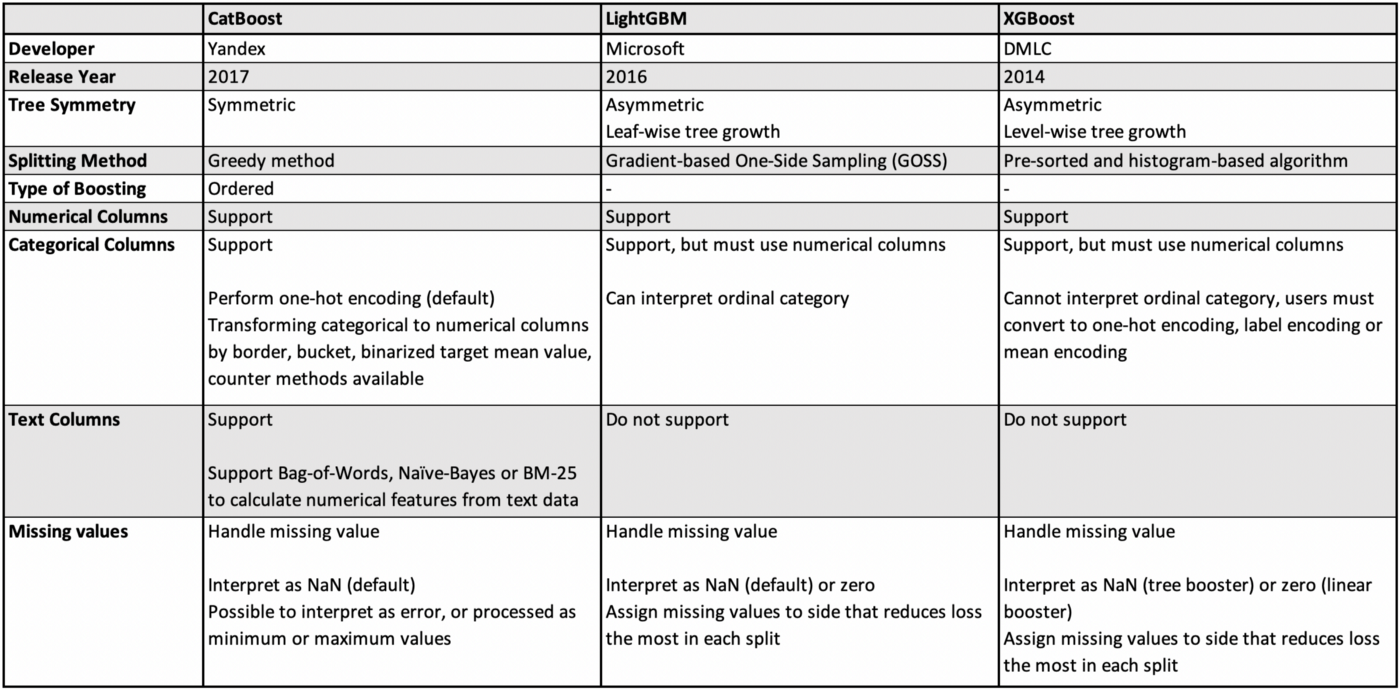
\includegraphics[scale=0.23]{xgb_cat_ligt.png}
\end{figure}
\end{frame}
\section{Results: Default x Optuna - 10min}
\subsection{Disclaimer}
\begin{frame}
\frametitle{Hyperparameter Space}
\textbf{learning\_rate , max\_depth, reg\_lambda}
\begin{gather*}
    LR = \{0.1,0.3\}\\
    MD = \{3,6\}\\
    RegL = \{0.01,0.05\}
\end{gather*}
\end{frame}
\begin{frame}
\frametitle{Hyperparameter Space}
\begin{table}[H]
\label{res:dia:2}
\centering
\begin{tabular}{|c|c|c|c|}
\hline
	& \textbf{XGBoost} &\textbf{CatBoost} & \textbf{LightGBM} \\
\hline
\textbf{AUC}	& 0.92598	& 0.89428	& 0.89406\\
\hline
\textbf{logloss}	& 2.17379	& 3.13992	& 2.89838\\
\hline
\textbf{KS}	& 0.85195	& 0.78856	& 0.78812 \\
\hline
\textbf{time (s)}	& 0.10825	& 1.05492	& 0.09304 \\
\hline
\end{tabular}
\caption{$LR=0.1$,$MD=3$,$Reg_L=0.01$ }
\end{table}
\begin{table}[H]
\label{res:dia:3}
\centering
\begin{tabular}{|c|c|c|c|}
\hline
	& \textbf{XGBoost} &\textbf{CatBoost} & \textbf{LightGBM} \\
\hline
\textbf{AUC}	& 0.92598	&0.90448	&0.92598\\
\hline
\textbf{logloss}	& 2.17379	&2.41531	&2.17379\\
\hline
\textbf{KS}	& 0.85195	& 0.80895 &	0.85195 \\
\hline
\textbf{time (s)}	& 0.11743&	1.00966&	0.08180 \\
\hline
\end{tabular}
\caption{$LR=0.3$,$MD=3$,$Reg_L=0.01$}
\end{table}
\end{frame}
\subsection{Diabetes Prediction}
\begin{frame}
\frametitle{Diabetes Prediction}
\begin{table}[H]
\centering
\begin{tabular}{|c|c|c|c|}
\hline
	& \textbf{XGBoost} &\textbf{CatBoost} & \textbf{LightGBM} \\
\hline
\textbf{AUC}	&0.93639	& 0.89655	& 0.92066 \\
\hline
\textbf{logloss}	& 1.69072 & 2.65684	& 2.29456 \\
\hline
\textbf{KS}	& 0.87278	& 0.79311	& 0.84131 \\
\hline
\textbf{time (s)}	& 0.17799 &	 1.78698 &	0.08261 \\
\hline
\end{tabular}
\caption{Default}\label{res:dia:1}
\end{table}
\begin{table}[H]
\centering
\begin{tabular}{|c|c|c|c|}
\hline
	& \textbf{XGBoost} &\textbf{CatBoost} & \textcolor{blue}{\textbf{LightGBM}} \\
\hline
\textbf{AUC}	& 0.97595	&0.981106	&0.98166\\
\hline
\textbf{logloss}	& 0.17300&	0.17327	&0.18599\\
\hline
\textbf{KS}	& 0.87821&	0.87799&	0.88320\\
\hline
$\delta_{AUC}$	& 4.22\% & 9.43\%	   &     6.52\% \\
\hline
$\delta_{KS}$	&   0.62 	&  10.70\% &	4.98\%\\
\hline
\end{tabular}
\caption{Optuna}\label{res:dia:op}
\end{table}
\end{frame}
% \begin{frame}
% \frametitle{Diabetes: XGBoost}
% \begin{figure}[H]
%  \label{fig:op:dia:trials:xgb}
%  \centering
%  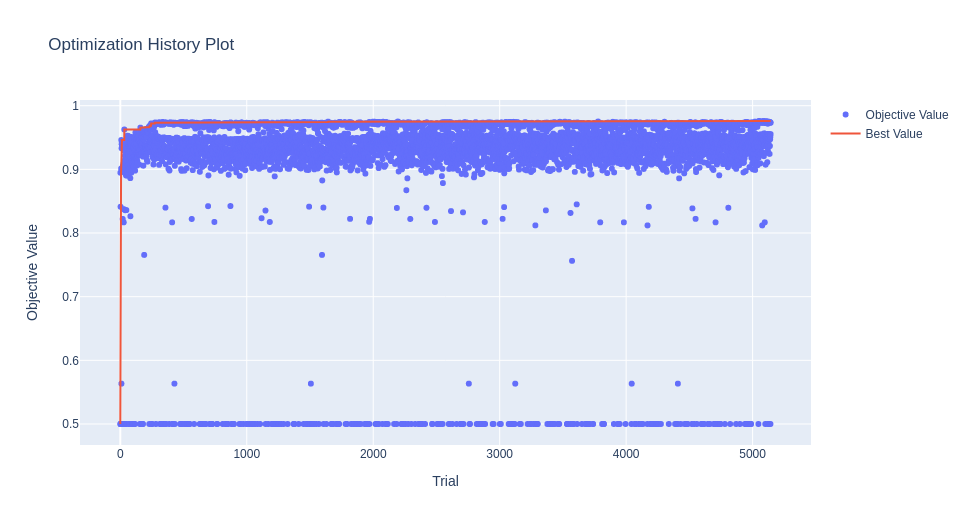
\includegraphics[scale=0.3]{optuna_xgboost_dia.png}
% \end{figure}
% \end{frame}
% \begin{frame}
% \frametitle{Diabetes: XGBoost}
% \begin{figure}[H]
%  \caption{Hiperparâmetros do XGBoost com maior importância no Optuna no dados de Diabetes.}.
%  \label{fig:op:dia:impo:xgb}
%  \centering
%  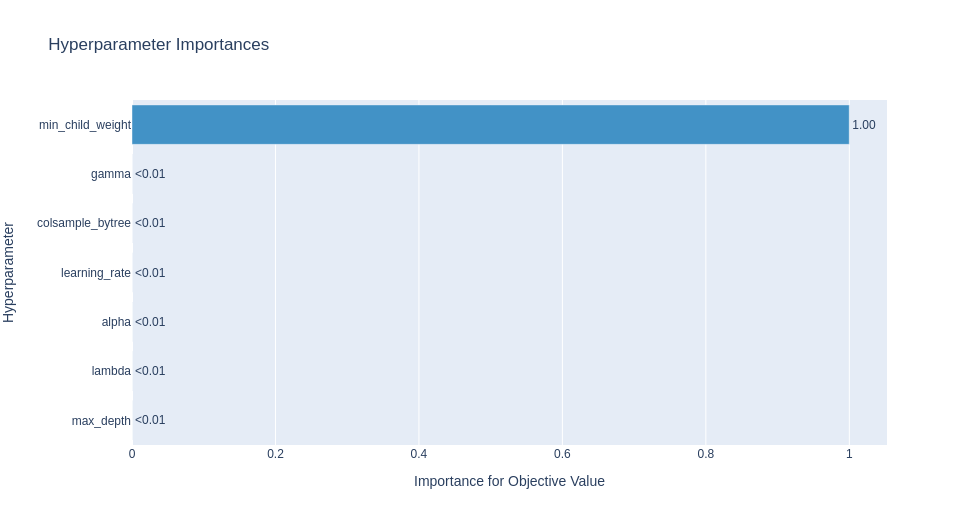
\includegraphics[scale=0.3]{importance_xgboost_dia.png}
% \end{figure}
% \end{frame}
% \begin{frame}
% \frametitle{Diabetes: XGBoost}
% 'min\_child\_weight': 1
% \begin{figure}[H]

%  \label{fig:op:dia:min:xgb}
%  \centering
%  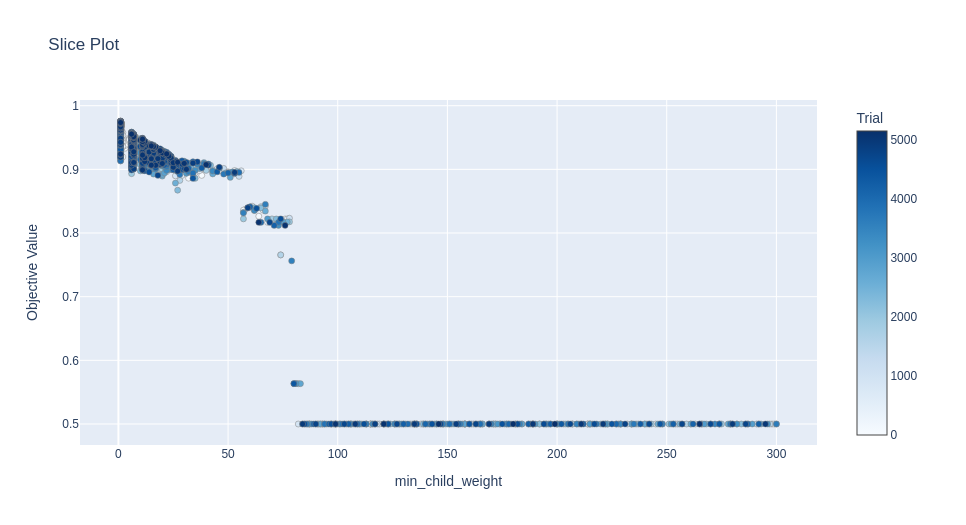
\includegraphics[scale=0.3]{optuna_xgboost_min_dia.png}
% \end{figure}
% \end{frame}
% \begin{frame}
% \frametitle{Diabetes: CatBoost}
% \begin{figure}[H]

%  \label{fig:op:dia:trials:cat}
%  \centering
%  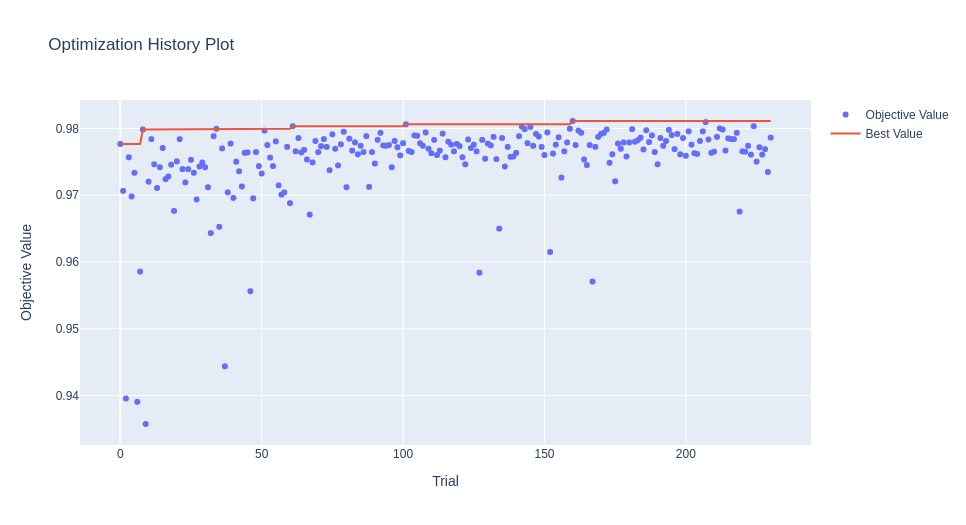
\includegraphics[scale=0.3]{optuna_catboost_dia.png}
% \end{figure}
% \end{frame}
% \begin{frame}
% \frametitle{Diabetes: CatBoost}
% \begin{figure}[H]

%  \label{fig:op:dia:impo:cat}
%  \centering
%  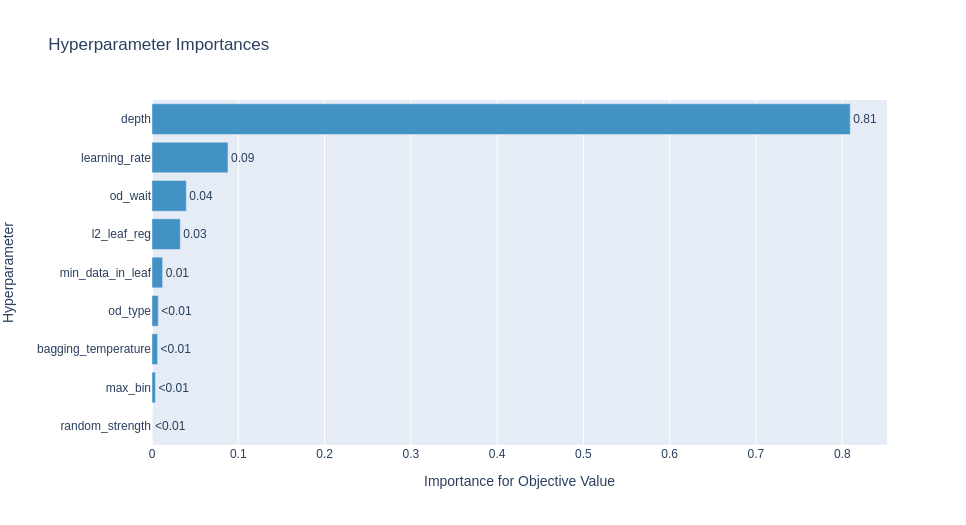
\includegraphics[scale=0.3]{importance_catboost_dia.png}
% \end{figure}
% \end{frame}
% \begin{frame}
% \frametitle{Diabetes: CatBoost}
% 'depth': 10
% \begin{figure}[H]

%  \label{fig:op:dia:dep:cat}
%  \centering
%  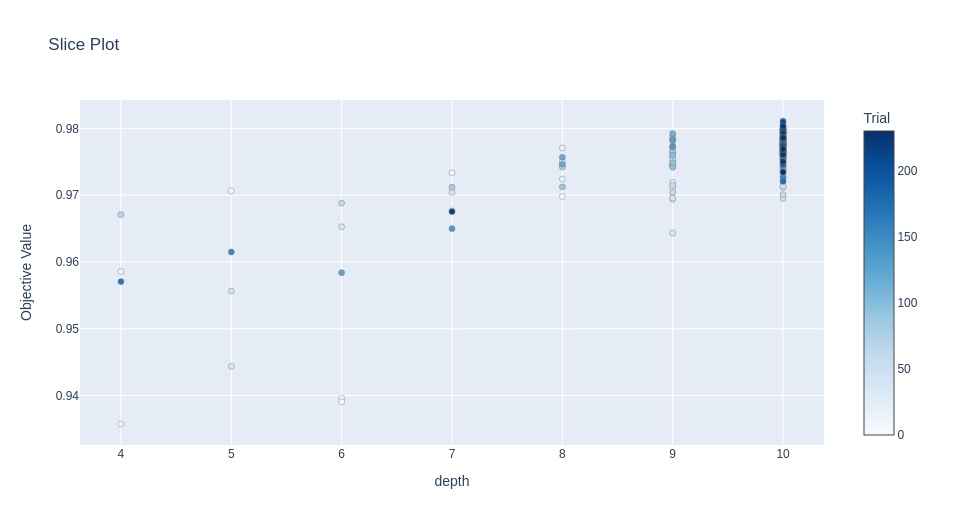
\includegraphics[scale=0.3]{optuna_cat_depth_dia.png}
% \end{figure}
% \end{frame}
% \begin{frame}
% \frametitle{Diabetes: CatBoost}
% 'learning\_rate': 0.005585552379158199
% \begin{figure}[H]

%  \label{fig:op:dia:len:cat}
%  \centering
%  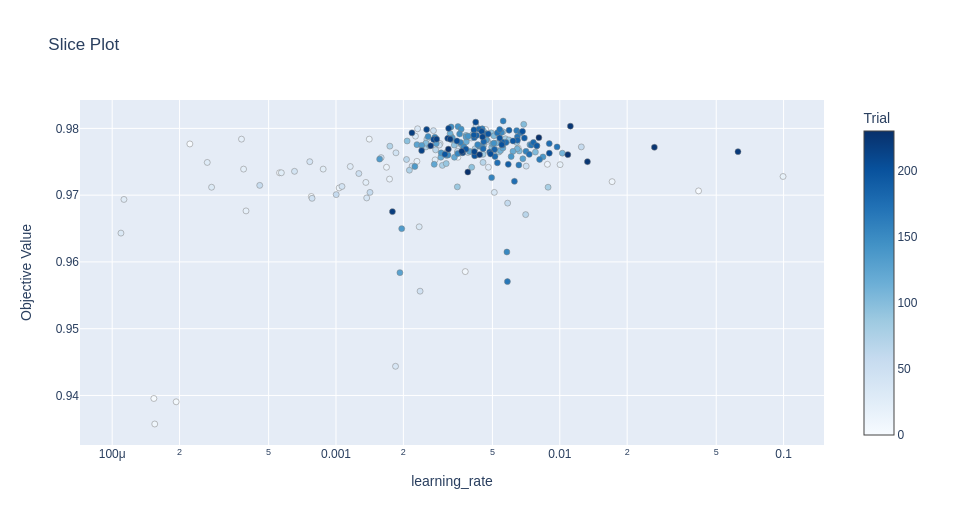
\includegraphics[scale=0.3]{optuna_cat_learnig_dia.png}
% \end{figure}
% \end{frame}
\begin{frame}
\frametitle{Diabetes: LightGBM}
\begin{figure}[H]

 \label{fig:op:dia:trials:lgbm}
 \centering
 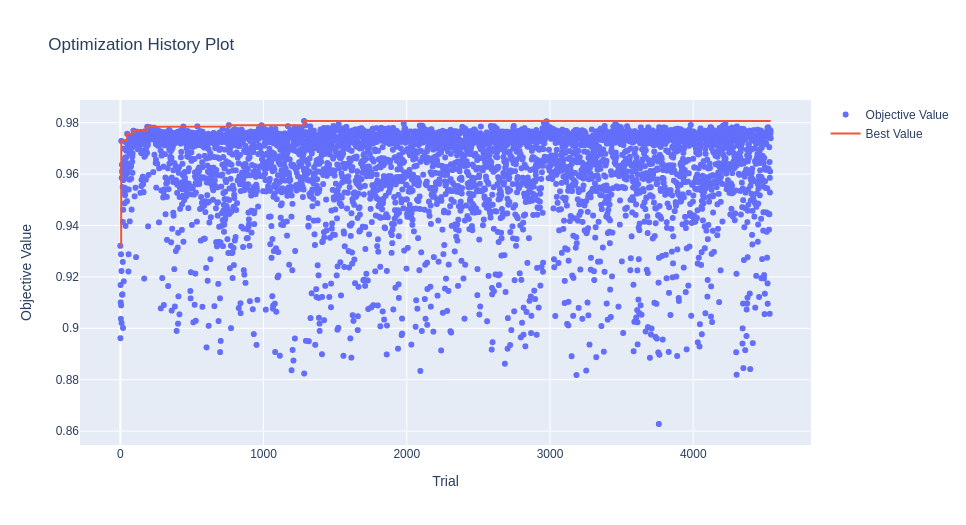
\includegraphics[scale=0.3]{optuna_lgbm_dia.png}
\end{figure}
\end{frame}
\begin{frame}
\frametitle{Diabetes: LightGBM}
\begin{figure}[H]

 \label{fig:op:dia:impo:lgbm}
 \centering
 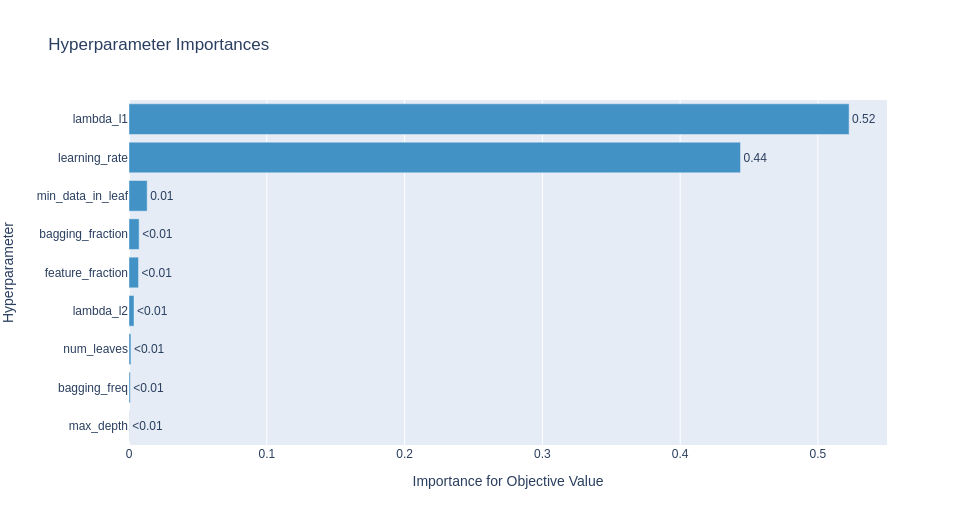
\includegraphics[scale=0.3]{importance_lgbm_dia.png}
\end{figure}
\end{frame}
\begin{frame}
\frametitle{Diabetes: LightGBM}
'lambda\_l1': 2.7481689793447196e-06
\begin{figure}[H]
 \label{fig:op:dia:lamb:lgbm}
 \centering
 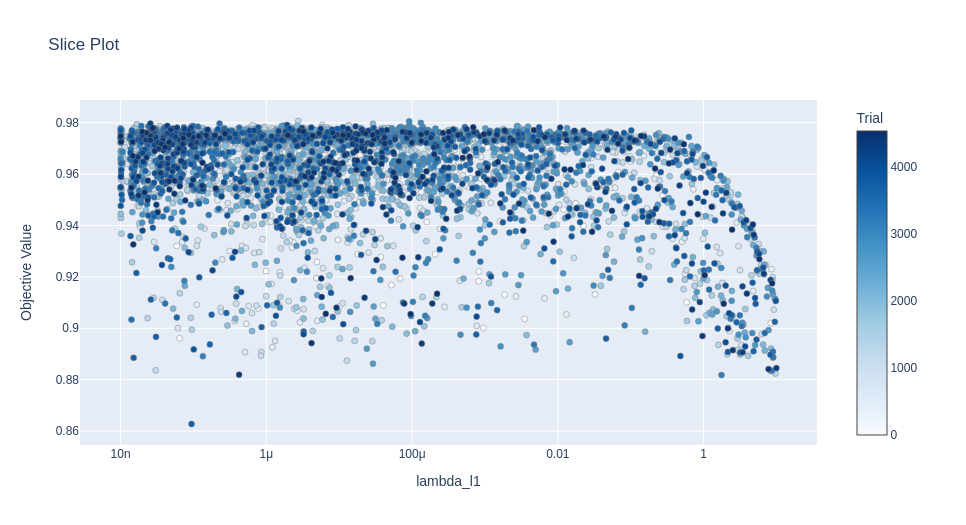
\includegraphics[scale=0.3]{optuna_lgbm_lambda_dia.png}
\end{figure}
\end{frame}
\begin{frame}
\frametitle{Diabetes: LightGBM}
'learning\_rate': 0.08425779644832665
\begin{figure}[H]
 \label{fig:op:dia:lamb:lgbm}
 \centering
 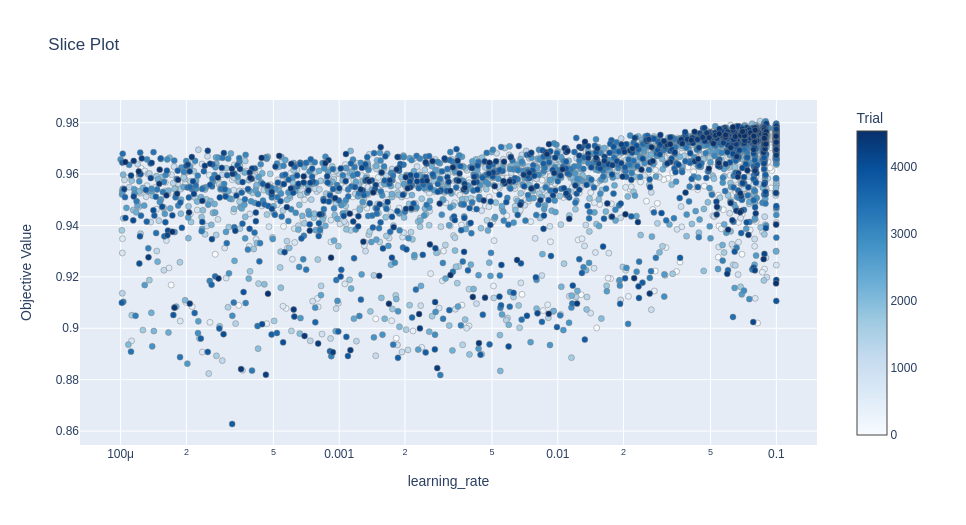
\includegraphics[scale=0.3]{optuna_lgbm_learn_dia.png}
\end{figure}
\end{frame}
\begin{frame}
\frametitle{Diabetes: SHAP LightGBM}
\begin{figure}[H]

 \label{fig:op:dia:lamb:lgbm}
 \centering
 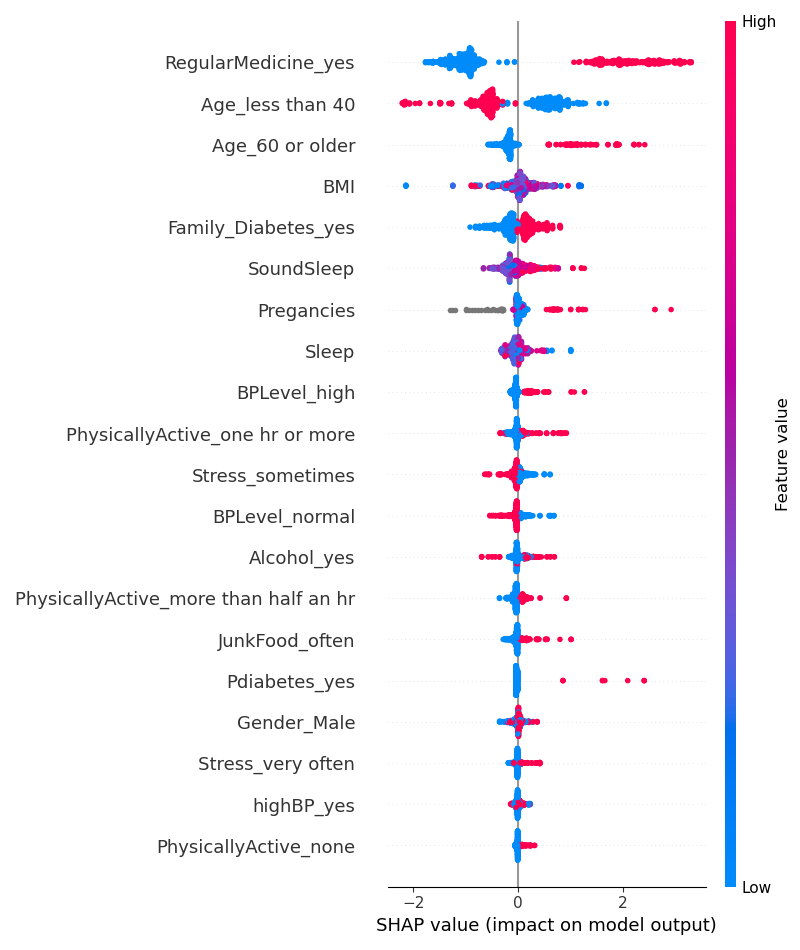
\includegraphics[scale=0.3]{shap_lgbm_diabete.png}
\end{figure}
\end{frame}
\subsection{Heart Failure Prediction}
\begin{frame}
\frametitle{Heart Failure Prediction}
\begin{table}[H]
\centering
\begin{tabular}{|c|c|c|c|}
\hline
	& \textbf{XGBoost} &\textbf{CatBoost} & \textbf{LightGBM} \\
\hline
\textbf{AUC}	& 0.84930&	0.90048&	0.86291\\
\hline
\textbf{logloss}	& 5.25595&	3.50396	&0.75538\\
\hline
\textbf{KS}	&0.69861	&0.80096	&0.72583\\
\hline
\textbf{time (s)}	& 0.13467	&1.41323	&0.06788 \\
\hline
\end{tabular}
\caption{Default}\label{res:dia:1}
\end{table}
\begin{table}[H]
\centering
\begin{tabular}{|c|c|c|c|}
\hline
	& \textcolor{blue}{\textbf{XGBoost}} &\textbf{CatBoost} & \textbf{LightGBM} \\
\hline
\hline
\textbf{AUC}	& 0.95852	&0.95019	&0.95835\\
\hline
\textbf{logloss}	& 0.28247	&0.30123	&0.29087\\
\hline
\textbf{KS}	&0.81598	&0.78680 &0.80945\\
\hline
$\delta_{AUC}$	& 12.51\%&	5.52\%	   &     11.06\% \\
\hline
$\delta_{KS}$	&    16.80\% 	&  -1.77\% &	11.52\%\\
\hline
\end{tabular}
\caption{Optuna}\label{res:dia:op}
\end{table}
\end{frame}
\begin{frame}
\frametitle{Heart Failure Prediction: XGBoost}
\begin{figure}[H]

 \label{fig:op:dia:lamb:lgbm}
 \centering
 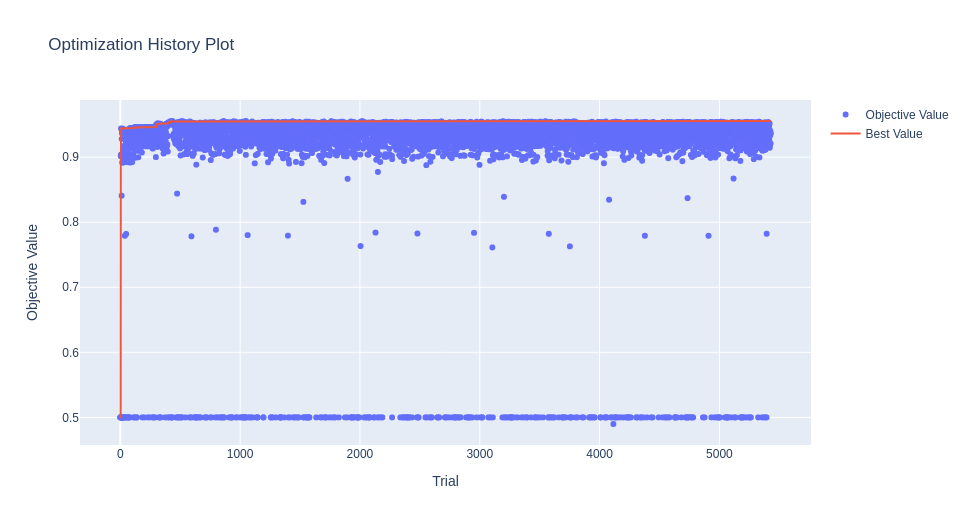
\includegraphics[scale=0.3]{optuna_xgboost_heart.png}
\end{figure}
\end{frame}
\begin{frame}
\frametitle{Heart Failure Prediction: XGBoost}
\begin{figure}[H]

 \label{fig:op:dia:lamb:lgbm}
 \centering
 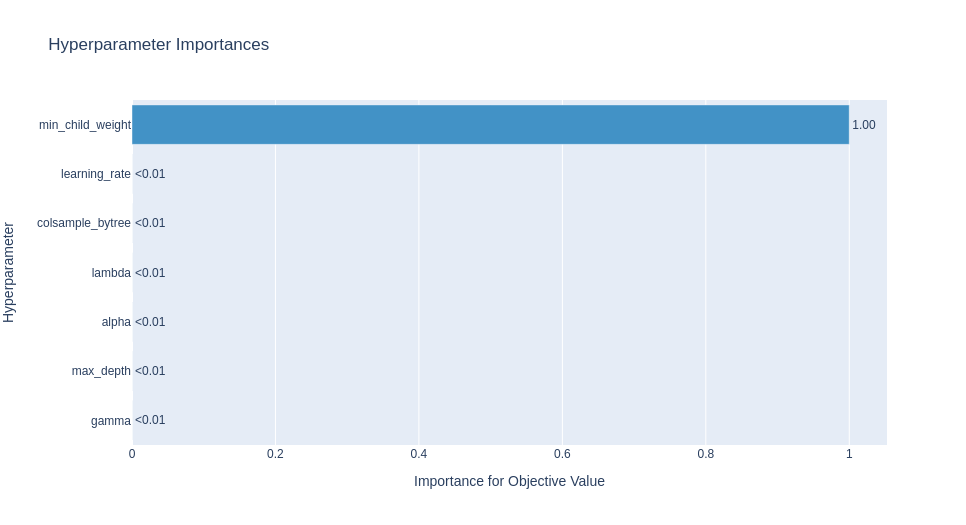
\includegraphics[scale=0.3]{optuna_xgboost_importance_heart.png}
\end{figure}
\end{frame}
\begin{frame}
\frametitle{Heart Failure Prediction: XGBoost}
'min\_child\_weight': 6
\begin{figure}[H]
 \centering
 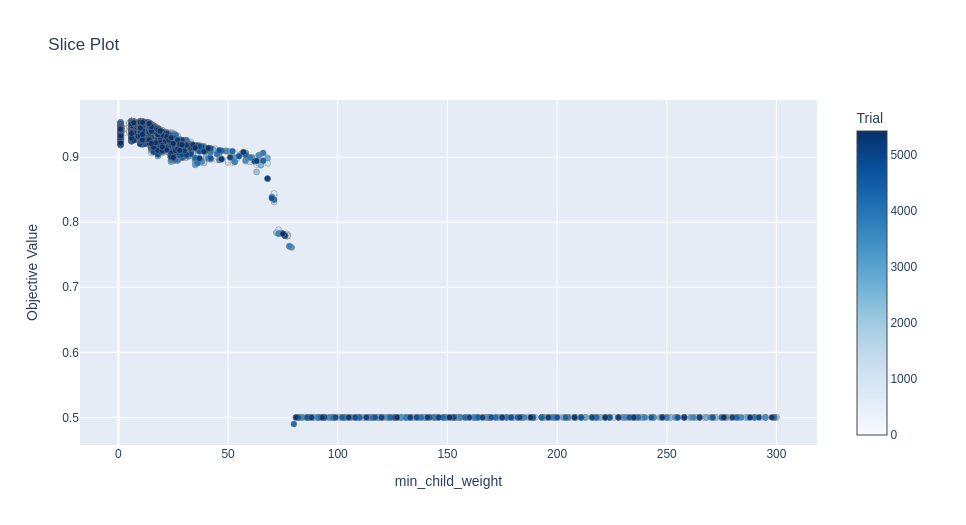
\includegraphics[scale=0.3]{optuna_xgboost_min_heart.png}
\end{figure}
\end{frame}
% \begin{frame}
% \frametitle{Heart Failure Prediction: CatBoost}
% \begin{figure}[H]

%  \label{fig:op:dia:lamb:lgbm}
%  \centering
%  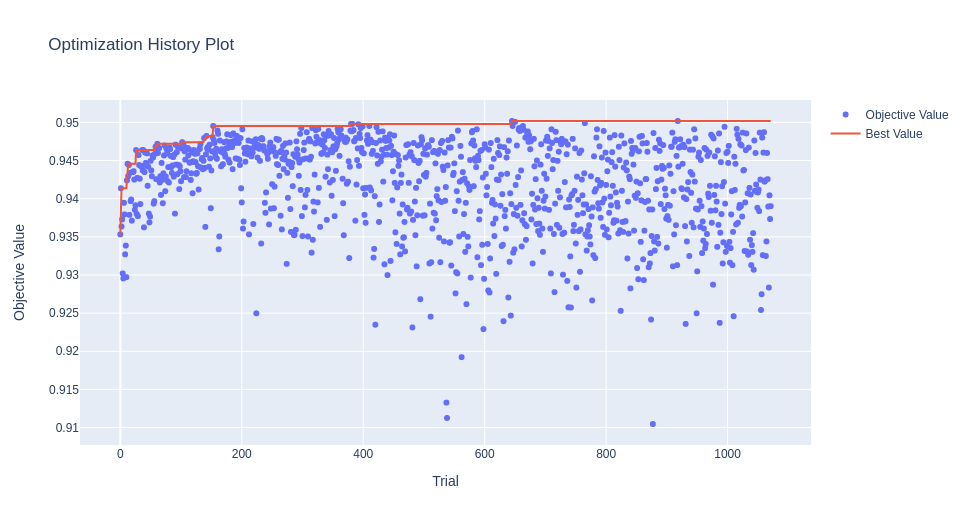
\includegraphics[scale=0.3]{optuna_catboost_heart.png}
% \end{figure}
% \end{frame}
% \begin{frame}
% \frametitle{Heart Failure Prediction: CatBoost}
% \begin{figure}[H]
%  \centering
%  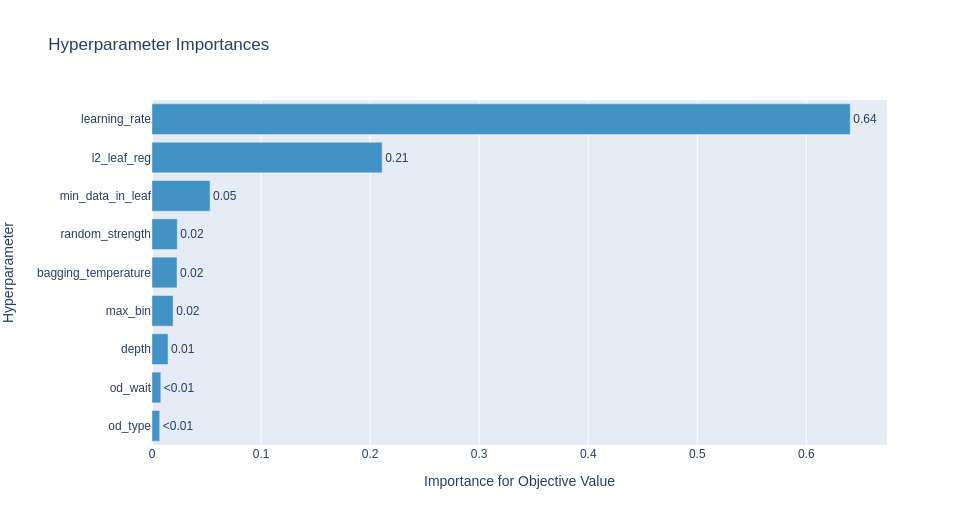
\includegraphics[scale=0.3]{optuna_catboost_importance_heart.png}
% \end{figure}
% \end{frame}
% \begin{frame}
% \frametitle{Heart Failure Prediction: CatBoost}
% 'learning\_rate': 0.006239961585898258
% \begin{figure}[H]
%  \centering
%  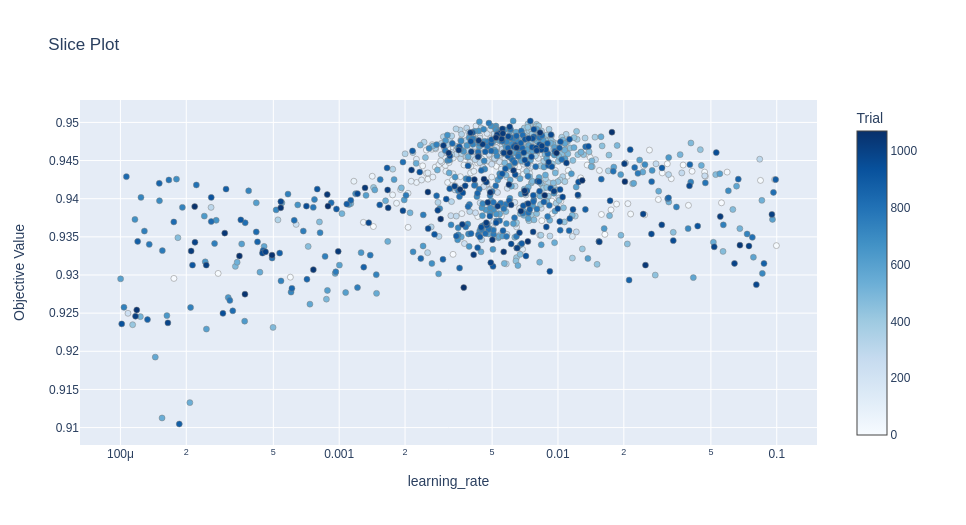
\includegraphics[scale=0.3]{optuna_catboost_learning_heart.png}
% \end{figure}
% \end{frame}
% \begin{frame}
% \frametitle{Heart Failure Prediction: CatBoost}
% 'l2\_leaf\_reg': 9.62802219566606
% \begin{figure}[H]
%  \label{fig:op:dia:lamb:lgbm}
%  \centering
%  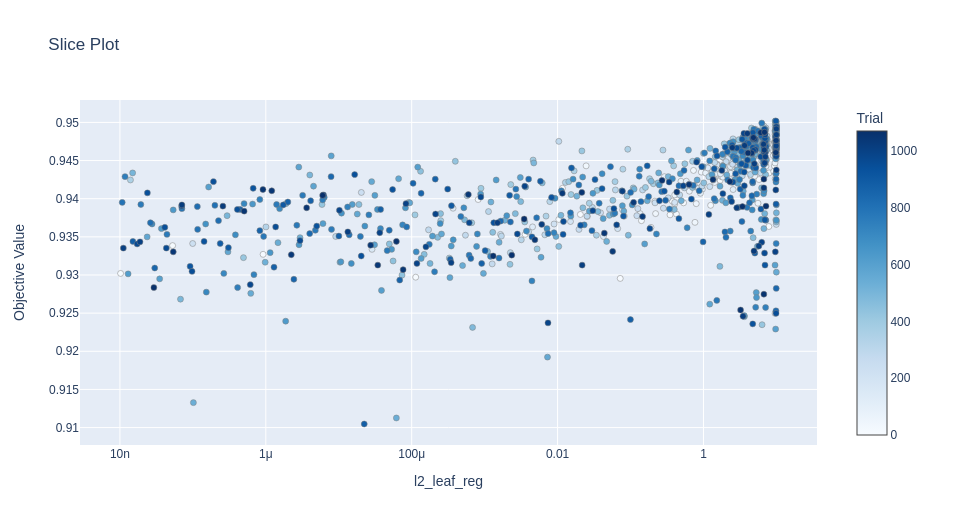
\includegraphics[scale=0.3]{optuna_catboost_l2_heart.png}
% \end{figure}
% \end{frame}
% \begin{frame}
% \frametitle{Heart Failure Prediction: LightGBM}
% \begin{figure}[H]
%  \label{fig:op:dia:lamb:lgbm}
%  \centering
%  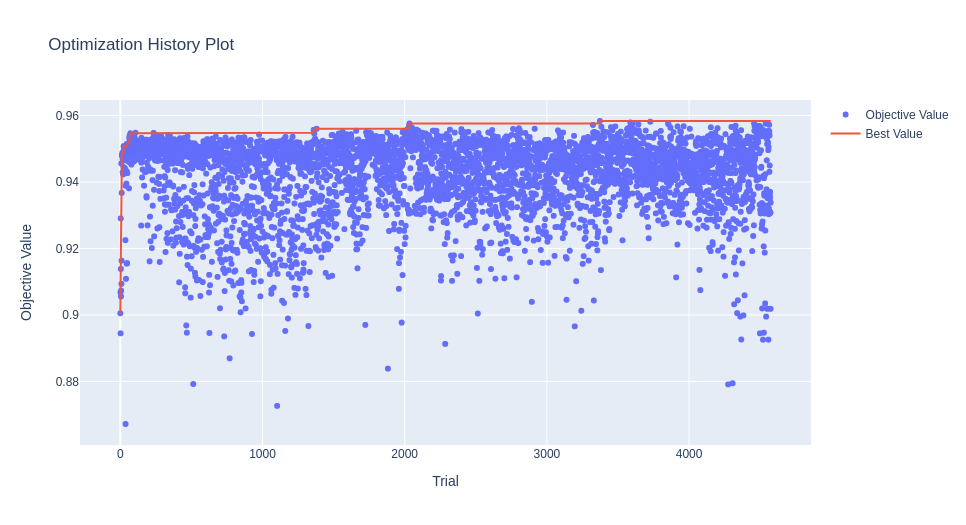
\includegraphics[scale=0.3]{optuna_lgbm_heart.png}
% \end{figure}
% \end{frame}
% \begin{frame}
% \frametitle{Heart Failure Prediction: LightGBM}
% \begin{figure}[H]
%  \label{fig:op:dia:lamb:lgbm}
%  \centering
%  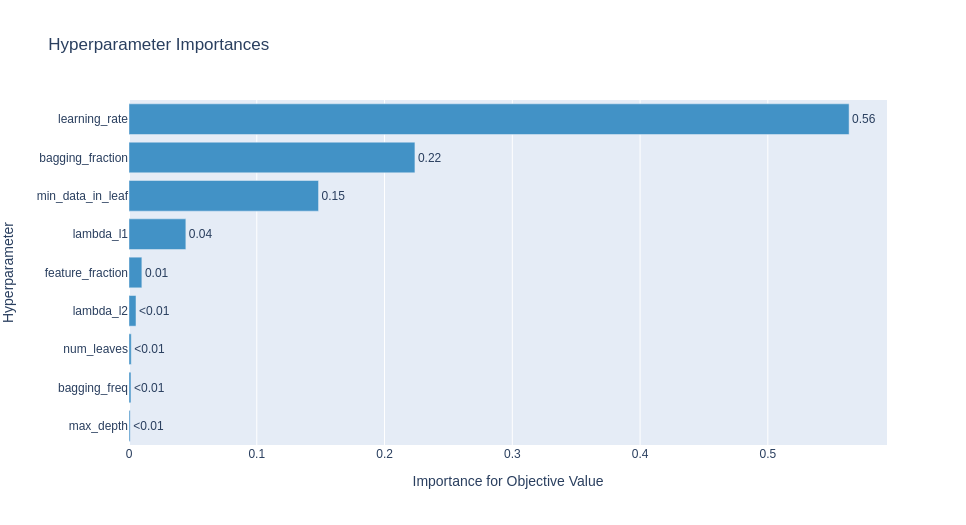
\includegraphics[scale=0.3]{optuna_lgbm_importance_heart.png}
% \end{figure}
% \end{frame}
% \begin{frame}
% \frametitle{Heart Failure Prediction: LightGBM}
% 'learning\_rate': 0.0765705960307223
% \begin{figure}[H]
%  \label{fig:op:dia:lamb:lgbm}
%  \centering
%  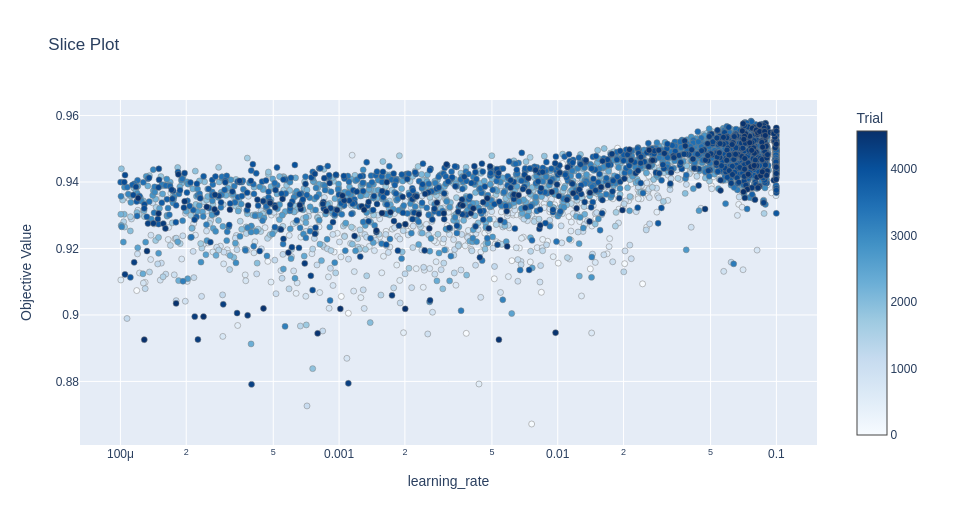
\includegraphics[scale=0.3]{optuna_lgbm_learning_heart.png}
% \end{figure}
% \end{frame}
% \begin{frame}
% \frametitle{Heart Failure Prediction: LightGBM}
% \begin{figure}[H]
%  \label{fig:op:dia:lamb:lgbm}
%  \centering
%  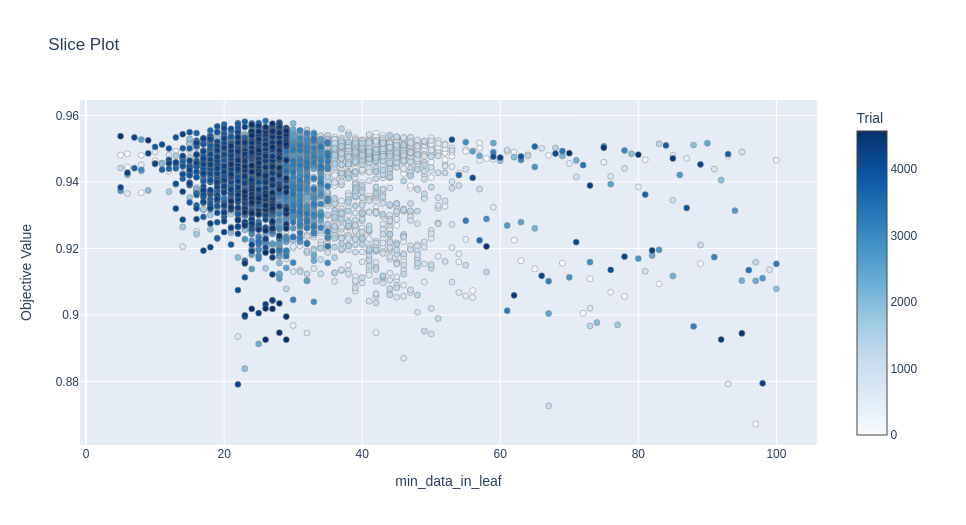
\includegraphics[scale=0.3]{optuna_lgbm_min_heart.png}
% \end{figure}
% \end{frame}
\begin{frame}
\frametitle{Heart Failure Prediction: SHAP XGBoost}
\begin{figure}[H]
 \centering
 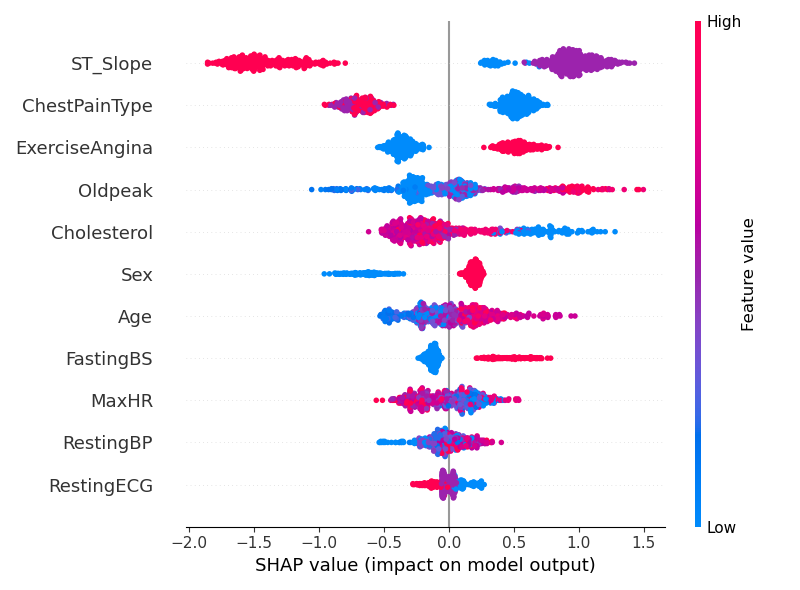
\includegraphics[scale=0.4]{shap_lgbm_heart.png}
\end{figure}
\end{frame}
\subsection{Kidney Stone Prediction}
\begin{frame}
\frametitle{Kidney Stone Prediction}
\begin{table}[H]
\centering
\begin{tabular}{|c|c|c|c|}
\hline
	& \textbf{XGBoost} &\textbf{CatBoost} & \textbf{LightGBM} \\
\hline
\textbf{AUC}	& 0.67857	&0.74286	&0.72857\\
\hline
\textbf{logloss}	& 10.07388	&8.63479	&8.63476\\
\hline
\textbf{KS}	&0.35714&	0.48571&	0.45714\\
\hline
\textbf{time (s)}	&0.10748	&0.27430	&0.09398 \\
\hline
\end{tabular}
\caption{Default}\label{res:dia:1}
\end{table}
\begin{table}[H]
\centering
\begin{tabular}{|c|c|c|c|}
\hline
	& \textbf{XGBoost} & \textcolor{blue}{\textbf{CatBoost}} & \textbf{LightGBM} \\
\hline
\textbf{AUC}	& 0.80000	&0.90000&	0.88571 \\
\hline
\textbf{logloss}	& 0.57024	& 0.96512 &	0.43693\\
\hline
\textbf{KS}	&0.51429&	0.71429	& 0.72857\\
\hline
$\delta_{AUC}$	& 31.76\%&	23.53\%	   &     21.57\% \\
\hline
$\delta_{KS}$	& 140.00\%     	&  56.26\% &	59.37\%\\
\hline
\end{tabular}
\caption{Optuna}\label{res:dia:op}
\end{table}
\end{frame}

% \begin{frame}
% \frametitle{Kidney Stone Prediction: XGBoost}
% \begin{figure}[H]
%  \centering
%  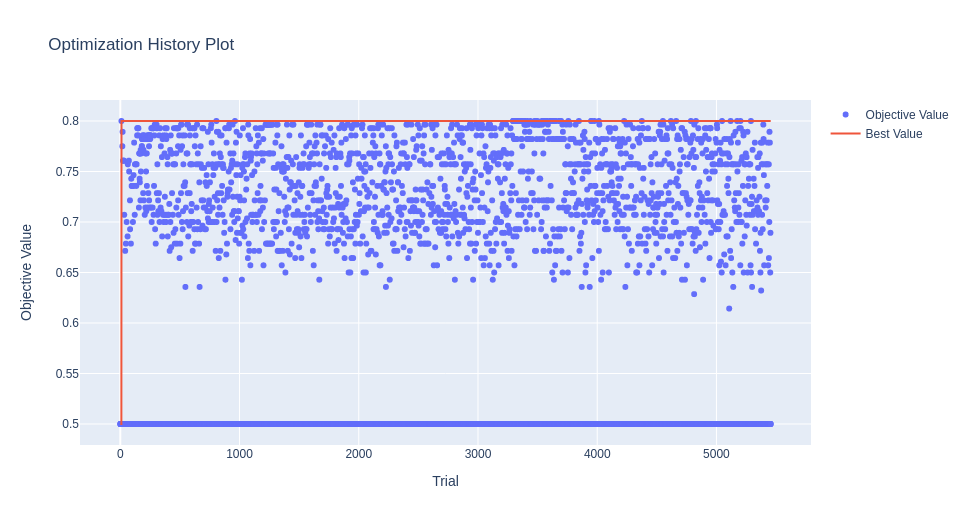
\includegraphics[scale=0.3]{optuna_xgboost_kindey.png}
% \end{figure}
% \end{frame}

% \begin{frame}
% \frametitle{Kidney Stone Prediction: XGBoost}
% \begin{figure}[H]
%  \centering
%  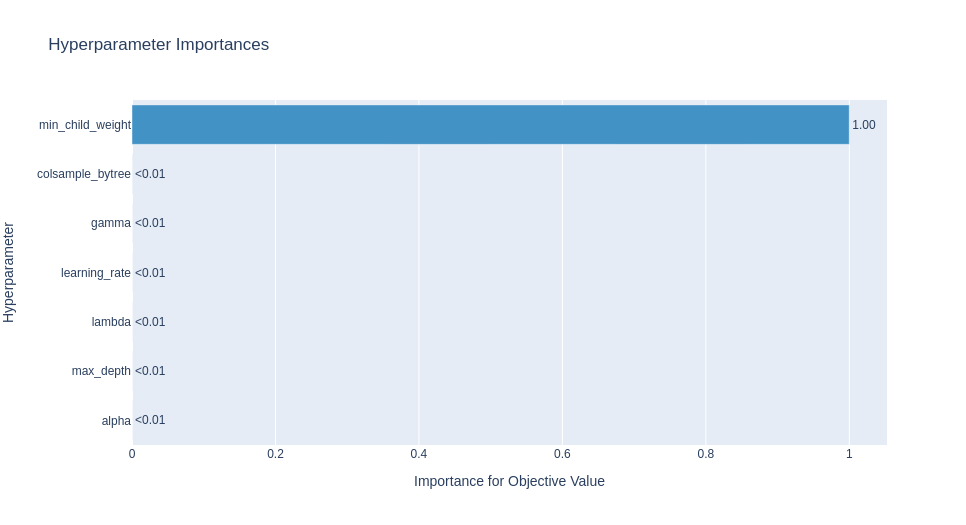
\includegraphics[scale=0.3]{optuna_xgboost_importance_kidney.png}
% \end{figure}
% \end{frame}

% \begin{frame}
% \frametitle{Kidney Stone Prediction: XGBoost}
% 'min\_child\_weight': 4
% \begin{figure}[H]
%  \centering
%  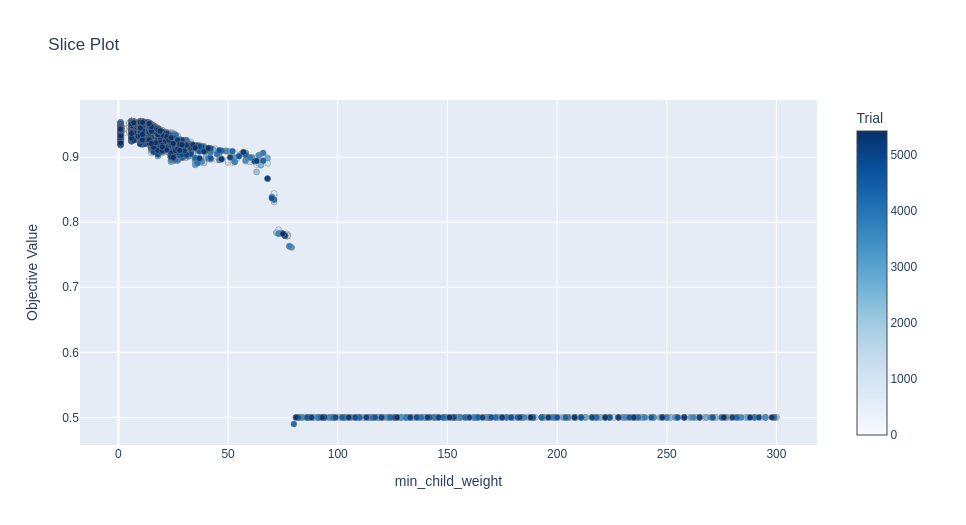
\includegraphics[scale=0.3]{optuna_xgboost_min_heart.png}
% \end{figure}
% \end{frame}

\begin{frame}
\frametitle{Kidney Stone Prediction: CatBoost}
\begin{figure}[H]
 \centering
 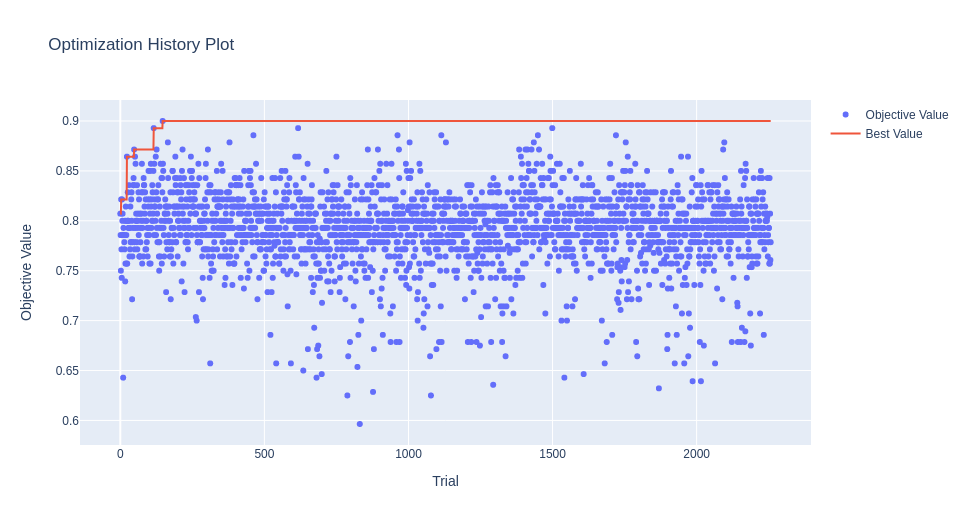
\includegraphics[scale=0.3]{optuna_catboost_kidney.png}
\end{figure}
\end{frame}

\begin{frame}
\frametitle{Kidney Stone Prediction: CatBoost}
\begin{figure}[H]
 \centering
 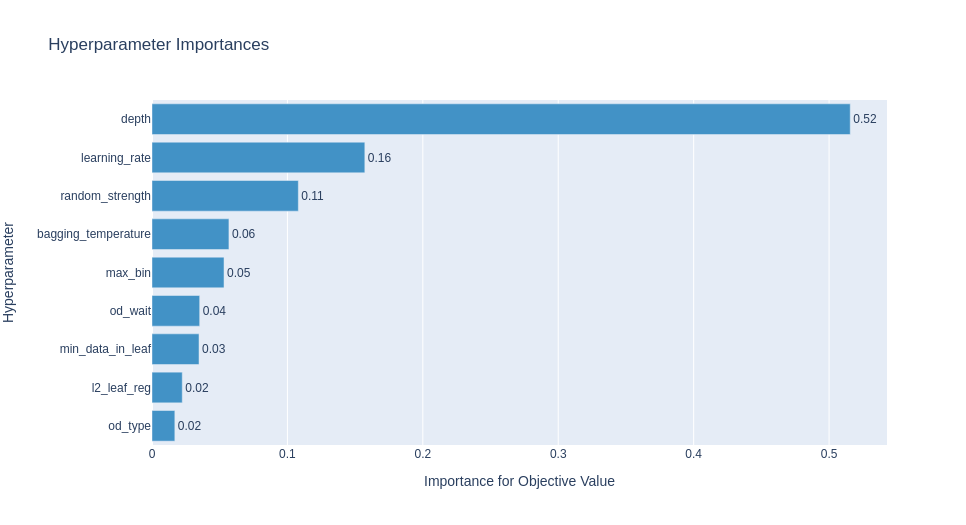
\includegraphics[scale=0.3]{optuna_catboost_importance_kidney.png}
\end{figure}
\end{frame}

\begin{frame}
\frametitle{Kidney Stone Prediction: CatBoost}
'depth': 5
\begin{figure}[H]
 \centering
 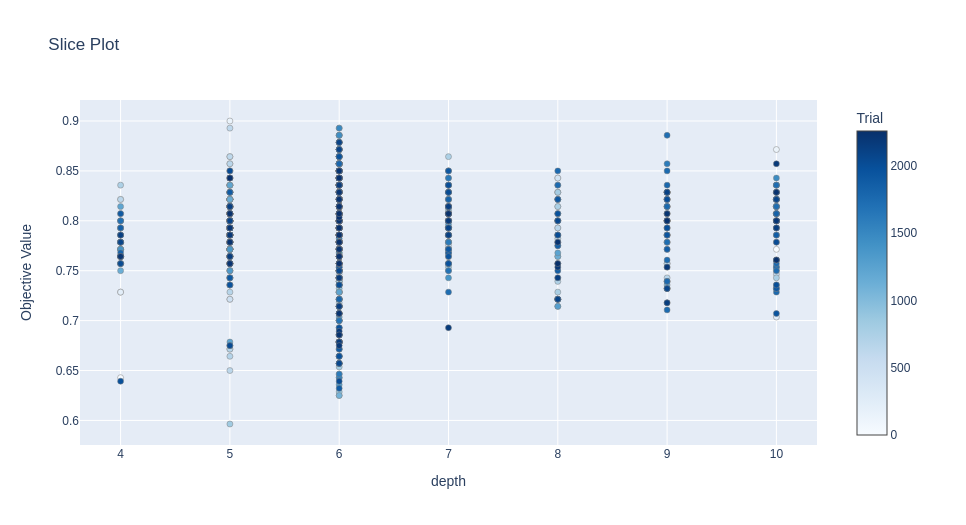
\includegraphics[scale=0.3]{opatuna_catboost_depth_kindey.png}
\end{figure}
\end{frame}

\begin{frame}
'learning\_rate': 0.07537894328903638
\frametitle{Kidney Stone Prediction: CatBoost}
\begin{figure}[H]
 \centering
 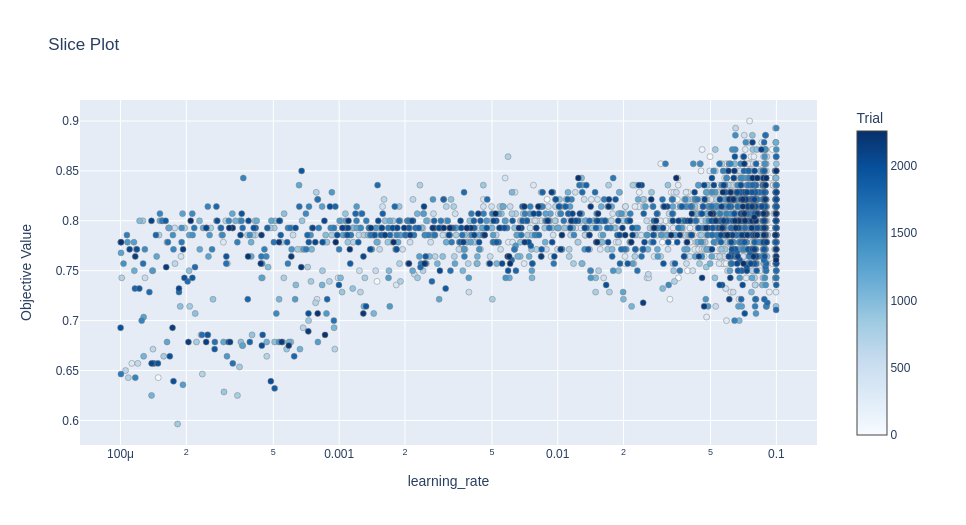
\includegraphics[scale=0.3]{optuna_learning_rate-catboost_kindey.png}
\end{figure}
\end{frame}

% \begin{frame}
% \frametitle{Kidney Stone Prediction: LightGBM}
% \begin{figure}[H]
%  \centering
%  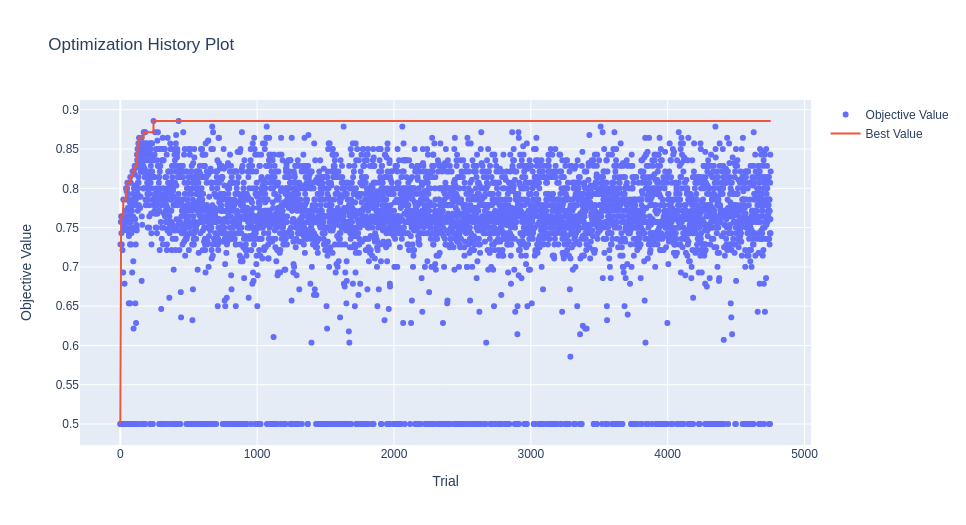
\includegraphics[scale=0.3]{optuna_lgbm_kikndey.png}
% \end{figure}
% \end{frame}

% \begin{frame}
% \frametitle{Kidney Stone Prediction: LightGBM}
% \begin{figure}[H]
%  \centering
%  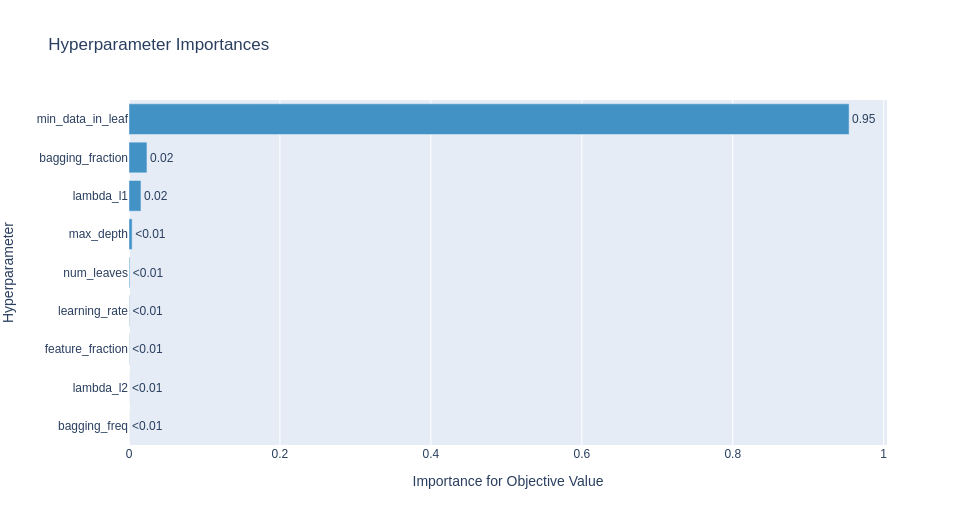
\includegraphics[scale=0.3]{optuna_lgbm_importance_kindey.png}
% \end{figure}
% \end{frame}

% \begin{frame}
% \frametitle{Kidney Stone Prediction: LightGBM}
% 'min\_data\_in\_leaf': 7
% \begin{figure}[H]
%  \centering
%  \includegraphics[scale=0.3]{optuna_min_lgbm_kindey.png}
% \end{figure}
% \end{frame}

\begin{frame}
\frametitle{Kidney Stone Prediction: SHAP CatBoost}
\begin{figure}[H]
 \centering
 \includegraphics[scale=0.5]{shap_lgbm_kidney.png}
\end{figure}
\end{frame}
\subsection{Breast Cancer Wisconsin Diagnostic}
\begin{frame}
\frametitle{Breast Cancer Wisconsin: XGBoost}
\begin{table}[H]
\centering
\begin{tabular}{|c|c|c|c|}
\hline
	& \textbf{XGBoost} &\textbf{CatBoost} & \textbf{LightGBM} \\
\hline
\textbf{AUC}	& 0.97950	&0.97156	&0.94511 \\
\hline
\textbf{logloss}	&0.60595	&0.80793&	1.81785 \\
\hline
\textbf{KS}	&0.95899	&0.94312	&0.89021 \\
\hline
\textbf{time (s)}	&0.14904	&2.72823	&0.08682 \\
\hline
\end{tabular}
\caption{Default}\label{res:dia:1}
\end{table}
\begin{table}[H]
\centering
\begin{tabular}{|c|c|c|c|}
\hline
	& \textbf{XGBoost} &\textbf{CatBoost} & \textcolor{blue}{\textbf{LightGBM}} \\
\hline
\textbf{AUC}	& 0.99882 &	0.99927 &0.99941 \\
\hline
\textbf{logloss}	& 0.11639	&0.04454 &	0.06708 \\
\hline
\textbf{KS}	&0.98413	&0.97487 &	0.98413 \\
\hline
$\delta_{AUC}$	& 1.97\%&	2.85\%	   &     5.75\% \\
\hline
$\delta_{KS}$	& 2.62\%    	&  3.37\% &	10.55\%\\
\hline
\end{tabular}
\caption{Optuna}\label{res:dia:op}
\end{table}
\end{frame}

% \begin{frame}
% \frametitle{Breast Cancer Wisconsin: XGBoost}
% \begin{figure}[H]
%  \centering
%  \includegraphics[scale=0.3]{optuna_xgboost_cancer.png}
% \end{figure}
% \end{frame}

% \begin{frame}
% \frametitle{Breast Cancer Wisconsin: XGBoost}
% \begin{figure}[H]
%  \centering
%  \includegraphics[scale=0.3]{optuna_xgboost_imporatnce_cancer.png}
% \end{figure}
% \end{frame}

% \begin{frame}
% \frametitle{Breast Cancer Wisconsin: XGBoost}
% 'min\_child\_weight': 15
% \begin{figure}[H]
%  \centering
%  \includegraphics[scale=0.3]{optuna_xgboost_min_cancer.png}
% \end{figure}
% \end{frame}

% \begin{frame}
% \frametitle{Breast Cancer Wisconsin: CatBoost}
% \begin{figure}[H]
%  \centering
%  \includegraphics[scale=0.3]{optuna_catboost_kidney.png}
% \end{figure}
% \end{frame}

% \begin{frame}
% \frametitle{Breast Cancer Wisconsin: CatBoost}
% \begin{figure}[H]
%  \centering
%  \includegraphics[scale=0.3]{optuna_catboost_imporatnce_cancer.png}
% \end{figure}
% \end{frame}

% \begin{frame}
% \frametitle{Breast Cancer Wisconsin: CatBoost}
% 'random\_strength': 5.267279748486068
% \begin{figure}[H]
%  \centering
%  \includegraphics[scale=0.3]{optuna_catboost_random_cancer.png}
% \end{figure}
% \end{frame}

% \begin{frame}
% 'learning\_rate': 0.014693012954604871
% \frametitle{Breast Cancer Wisconsin: CatBoost}
% \begin{figure}[H]
%  \centering
%  \includegraphics[scale=0.3]{optuna_catboost_learning_cancer.png}
% \end{figure}
% \end{frame}

\begin{frame}
\frametitle{Breast Cancer Wisconsin: LightGBM}
\begin{figure}[H]
 \centering
 \includegraphics[scale=0.3]{optuna_lgbm_cancer.png}
\end{figure}
\end{frame}

\begin{frame}
\frametitle{Breast Cancer Wisconsin: LightGBM}
\begin{figure}[H]
 \centering
 \includegraphics[scale=0.3]{optuna_lgbm_importance_cancer.png}
\end{figure}
\end{frame}

\begin{frame}
\frametitle{Breast Cancer Wisconsin: LightGBM}
'min\_data\_in\_leaf': 66
\begin{figure}[H]
 \centering
 \includegraphics[scale=0.3]{optuna_lgbm_min_cancer.png}
\end{figure}
\end{frame}
\begin{frame}
\frametitle{Breast Cancer Wisconsin: LightGBM}
'learning\_rate': 0.07615521372640538 
\begin{figure}[H]
 \centering
 \includegraphics[scale=0.3]{optuna_lgbm_learning_cancer.png}
\end{figure}
\end{frame}

\begin{frame}
\frametitle{Breast Cancer Wisconsin: SHAP LightGBM}
\begin{figure}[H]
 \centering
 \includegraphics[scale=0.3]{shap_cancer.png}
\end{figure}
\end{frame}










 % A subsection can be created just before a set of slides with a common theme to further break down your presentation into chunks

% \begin{frame}
% \frametitle{Paragraphs of Text}
% Sed iaculis dapibus gravida. Morbi sed tortor erat, nec interdum arcu. Sed id lorem lectus. Quisque viverra augue id sem ornare non aliquam nibh tristique. Aenean in ligula nisl. Nulla sed tellus ipsum. Donec vestibulum ligula non lorem vulputate fermentum accumsan neque mollis.\\~\\

% Sed diam enim, sagittis nec condimentum sit amet, ullamcorper sit amet libero. Aliquam vel dui orci, a porta odio. Nullam id suscipit ipsum. Aenean lobortis commodo sem, ut commodo leo gravida vitae. Pellentesque vehicula ante iaculis arcu pretium rutrum eget sit amet purus. Integer ornare nulla quis neque ultrices lobortis. Vestibulum ultrices tincidunt libero, quis commodo erat ullamcorper id.
% \end{frame}

% %------------------------------------------------

% \begin{frame}
% \frametitle{Bullet Points}
% \begin{itemize}
% \item Lorem ipsum dolor sit amet, consectetur adipiscing elit
% \item Aliquam blandit faucibus nisi, sit amet dapibus enim tempus eu
% \item Nulla commodo, erat quis gravida posuere, elit lacus lobortis est, quis porttitor odio mauris at libero
% \item Nam cursus est eget velit posuere pellentesque
% \item Vestibulum faucibus velit a augue condimentum quis convallis nulla gravida
% \end{itemize}
% \end{frame}

% %------------------------------------------------

% \begin{frame}
% \frametitle{Blocks of Highlighted Text}
% \begin{block}{Block 1}
%  curva ROC é calculada pelo gráfico de \textit{Taxa de Verdadeiros Positivos (TVP)}, ou Sensibilidade, versus \textit{Taxa de Falso Positivos (TFP)}, ou Especificidade.
% \end{block}

% \begin{block}{Block 2}
% Pellentesque sed tellus purus. Class aptent taciti sociosqu ad litora torquent per conubia nostra, per inceptos himenaeos. Vestibulum quis magna at risus dictum timer eu vitae velit.
% \end{block}

% \begin{block}{Block 3}
% Suspendisse tincidunt sagittis gravida. Curabitur condimentum, enim sed venenatis rutrum, ipsum neque consectetur orci, sed blandit justo nisi ac lacus.
% \end{block}
% \end{frame}

% %------------------------------------------------

% \begin{frame}
% \frametitle{Multiple Columns}
% \begin{columns}[c] % The "c" option specifies centered vertical alignment while the "t" option is used for top vertical alignment

% \column{.45\textwidth} % Left column and width
% \textbf{Heading}
% \begin{enumerate}
% \item Statement
% \item Explanation
% \item Example
% \end{enumerate}

% \column{.5\textwidth} % Right column and width
% Lorem ipsum dolor sit amet, consectetur adipiscing elit. Integer lectus nisl, ultricies in feugiat rutrum, porttitor sit amet augue. Aliquam ut tortor mauris. Sed volutpat ante purus, quis accumsan dolor.

% \end{columns}
% \end{frame}

% %------------------------------------------------

% %------------------------------------------------

% \begin{frame}
% \frametitle{Table}
% \begin{table}
% \begin{tabular}{l l l}
% \toprule
% \textbf{Treatments} & \textbf{Response 1} & \textbf{Response 2}\\
% \midrule
% Treatment 1 & 0.0003262 & 0.562 \\
% Treatment 2 & 0.0015681 & 0.910 \\
% Treatment 3 & 0.0009271 & 0.296 \\
% \bottomrule
% \end{tabular}
% \caption{Table caption}
% \end{table}
% \end{frame}

% %------------------------------------------------

% \begin{frame}
% \frametitle{Theorem}
% \begin{theorem}[Mass--energy equivalence]
% $E = mc^2$
% \end{theorem}
% \end{frame}

% %------------------------------------------------

% \begin{frame}[fragile] % Need to use the fragile option when verbatim is used in the slide
% \frametitle{Verbatim}
% \begin{example}[Theorem Slide Code]
% \begin{verbatim}
% \begin{frame}
% \frametitle{Theorem}
% \begin{theorem}[Mass--energy equivalence]
% $E = mc^2$
% \end{theorem}
% \end{frame}\end{verbatim}
% \end{example}
% \end{frame}

% %------------------------------------------------

% \begin{frame}
% \frametitle{Figure}
% Uncomment the code on this slide to include your own image from the same directory as the template .TeX file.
% %\begin{figure}
% %\includegraphics[width=0.8\linewidth]{test}
% %\end{figure}
% \end{frame}

% %------------------------------------------------

% \begin{frame}[fragile] % Need to use the fragile option when verbatim is used in the slide
% \frametitle{Citation}
% An example of the \verb|\cite| command to cite within the presentation:\\~

% This statement requires citation \cite{p1}.
% \end{frame}

% %------------------------------------------------

\begin{frame}
\frametitle{References}
\footnotesize{
\begin{thebibliography}{99} % Beamer does not support BibTeX so references must be inserted manually as below
\bibitem[Smith, 2012]{p1} Trevor Hastie and Robert Tibshirani and Jerome Friedman (2009)
\newblock The Elements of Statistical Learning 
\bibitem[Smith, 2012]{p1} Stuart J. Russell and Peter Norvig (2021)
\newblock Artificial Intelligence: A Modern Approach, Global Edition
\bibitem[Smith, 2012]{p1} Max Kuhn and Kjell Johnson (2013)
\newblock Applied Predictive Modeling
% \newblock \emph{Journal Name} 12(3), 45 -- 678.
\end{thebibliography}
}
\end{frame}

% %------------------------------------------------

% \begin{frame}
% \Huge{\centerline{The End}}
% \end{frame}

% %----------------------------------------------------------------------------------------

\end{document}

